
%%%%%%%%%%%%%%%%%%%%%%%%%%%%%%%%%%%%%%%%%%%%%%%%%%%%%%%%%%%%%%%%%%%%%%%%%%%%%%%%
%% ************************************************************************** %%
%% *                                Settings                                * %%
%% ************************************************************************** %%
%%%%%%%%%%%%%%%%%%%%%%%%%%%%%%%%%%%%%%%%%%%%%%%%%%%%%%%%%%%%%%%%%%%%%%%%%%%%%%%%
\documentclass{tron}

\loadglsentries{gls}
\glsaddall
\addbibresource{reference}
\usepackage{xcolor}  % Coloured text etc.
% fancy note style
% STYLE NOTES : v2.0
% additional fancy boxes
\usepackage[framemethod=TikZ]{mdframed}
%\usepackage{amsthm}

% gray color indicates [OPTIONAL READING]

%%%%%%%%%%%%%%%%%%%%%%%%%%%%%%
%Note
\newenvironment{note}[3][]{%
	\ifstrempty{#1}%
	{\mdfsetup{%
	frametitle={%
	\tikz[baseline=(current bounding box.east),outer sep=0pt]
	\node[anchor=east,rectangle,fill=#2]
	{\strut Note};}}
	}%
	{\mdfsetup{%
	frametitle={%
	\tikz[baseline=(current bounding box.east),outer sep=0pt]
	\node[anchor=east,rectangle,fill=#2]
	{\strut #1};}}%
	}%
	\mdfsetup{innertopmargin=0pt,skipabove=5pt,linecolor=#2,%
		linewidth=2pt,topline=true,%
		frametitleaboveskip=\dimexpr-\ht\strutbox\relax,
		backgroundcolor={white!90!#2}}
	\begin{mdframed}[]\relax%
	\label{#3}}{\end{mdframed}
}
\Crefname{note}{Note}{notes}

\newcommand{\createnoteenv}[6]{
	\refstepcounter{#6}%
	\ifstrempty{#1}%
	{\mdfsetup{%
	frametitle={%
	\tikz[baseline=(current bounding box.east),outer sep=0pt]
	\node[anchor=east,rectangle,fill=#3]
	{\strut #4~#5};}}
	}%
	{
		\mdfsetup{%
			frametitle={%
				\tikz[baseline=(current bounding box.east),outer sep=0pt]
				\node[anchor=east,rectangle,fill=#3]
				{\strut #4~#5:~#1};
			}
		}%
	}%
	\mdfsetup{innertopmargin=0pt,skipabove=5pt,linecolor=#3,%
	linewidth=2pt,topline=true,%
	frametitleaboveskip=\dimexpr-\ht\strutbox\relax,
	backgroundcolor={white!90!#3}}
	\begin{mdframed}[]\relax%
	\label{#2}
}

%%%%%%%%%%%%%%%%%%%%%%%%%%%%%%
%Definition
\newcounter{definition}[section] \setcounter{definition}{0}
\renewcommand{\thedefinition}{\arabic{section}.\arabic{definition}}
\newenvironment{definition}[2][]{%
	\createnoteenv{#1}{#2}{blue!40}{Definition}{\thedefinition}{definition}%
}{\end{mdframed}}
\newenvironment{definition*}[2][]{%
	\createnoteenv{#1}{#2}{gray!40}{Definition}{\thedefinition}{definition}%
}{\end{mdframed}}
\Crefname{definition}{Definition}{definitions}


%%%%%%%%%%%%%%%%%%%%%%%%%%%%%%
%theoremrem
\newcounter{theorem}[section] \setcounter{theorem}{0}
\renewcommand{\thetheorem}{\arabic{section}.\arabic{theorem}}
\newenvironment{theorem}[2][]{%
	\createnoteenv{#1}{#2}{cyan!40}{Theorem}{\thetheorem}{theorem}%
}{\end{mdframed}}
\newenvironment{theorem*}[2][]{%
	\createnoteenv{#1}{#2}{gray!40}{Theorem}{\thetheorem}{theorem}%
}{\end{mdframed}}
\Crefname{theorem}{Theorem}{theorems}

%%%%%%%%%%%%%%%%%%%%%%%%%%%%%%
%Proof
\newcounter{proof}[section]\setcounter{proof}{0}
\renewcommand{\theproof}{\arabic{section}.\arabic{proof}}
\newenvironment{proof}[2][]{%
	\createnoteenv{#1}{#2}{red!20}{Proof}{\theproof}{proof}%
}{\end{mdframed}}
\newenvironment{proof*}[2][]{%
	\createnoteenv{#1}{#2}{gray!40}{Proof}{\theproof}{proof}%
}{\end{mdframed}}
\Crefname{proof}{Proof}{proofs}


%%%%%%%%%%%%%%%%%%%%%%%%%%%%%%
%Alert
\newcounter{alert}[section]\setcounter{alert}{0}
\renewcommand{\thealert}{\arabic{section}.\arabic{alert}}
\newenvironment{alert}[2][]{%
	\createnoteenv{#1}{#2}{red!80}{Alert}{\thealert}{alert}%
}{\end{mdframed}}
\newenvironment{alert*}[2][]{%
	\createnoteenv{#1}{#2}{gray!40}{Alert}{\thealert}{alert}%
}{\end{mdframed}}
\Crefname{alert}{Alert}{alerts}

%%%%%%%%%%%%%%%%%%%%%%%%%%%%%%
%Answer
\newcounter{answer}[section]\setcounter{answer}{0}
\renewcommand{\theanswer}{\arabic{section}.\arabic{answer}}
\newenvironment{answer}[2][]{%
	\createnoteenv{#1}{#2}{orange!60}{Answer}{\theanswer}{answer}%
}{\end{mdframed}}
\newenvironment{answer*}[2][]{%
	\createnoteenv{#1}{#2}{gray!40}{Answer}{\theanswer}{answer}%
}{\end{mdframed}}
\Crefname{answer}{Answer}{answers}

%%%%%%%%%%%%%%%%%%%%%%%%%%%%%%
%Remark
\newcounter{remark}[section]\setcounter{remark}{0}
\renewcommand{\theremark}{\arabic{section}.\arabic{remark}}
\newenvironment{remark}[2][]{%
	\createnoteenv{#1}{#2}{orange!40}{Remark}{\theremark}{remark}%
}{\end{mdframed}}
\newenvironment{remark*}[2][]{%
	\createnoteenv{#1}{#2}{gray!40}{Remark}{\theremark}{remark}%
}{\end{mdframed}}
\Crefname{remark}{Remark}{remarks}


%%%%%%%%%%%%%%%%%%%%%%%%%%%%%%%
%%Example
%\newcounter{example}[section]\setcounter{example}{0}
%\renewcommand{\theexample}{\arabic{section}.\arabic{example}}
%\newenvironment{example}[2][]{%
%	\createnoteenv{#1}{#2}{blue!40!cyan!20}{Example}{\theexample}{example}%
%}{\end{mdframed}}
%\newenvironment{example*}[2][]{%
%	\createnoteenv{#1}{#2}{gray!40}{Example}{\theexample}{example}%
%}{\end{mdframed}}

%%%%%%%%%%%%%%%%%%%%%%%%%%%%%%
%Algorithm
\newcounter{algo}[section]\setcounter{algo}{0}
\renewcommand{\thealgo}{\arabic{algo}.\arabic{algo}}
\newenvironment{algo}[2][]{%
	\createnoteenv{#1}{#2}{yellow!90!brown!60}{Algorithm}{\thealgo}{algo}%
}{\end{mdframed}}
\newenvironment{algo*}[2][]{%
	\createnoteenv{#1}{#2}{gray!40}{Algorithm}{\thealgo}{algo}%
}{\end{mdframed}}
\Crefname{algo}{Algorithm}{algos}

%%%%%%%%%%%%%%%%%%%%%%%%%%%%%%
% CS480 - Exercise
%\setlength{\parskip}{1cm}
%\setlength{\parindent}{1cm}

%\tikzstyle{titregris} =
%[draw=gray,fill=white, shading = exersicetitle, %
%text=gray, rectangle, rounded corners, right,minimum height=.3cm]
%\pgfdeclarehorizontalshading{exersicebackground}{100bp}
%{color(0bp)=(green!40); color(100bp)=(black!5)}
%\pgfdeclarehorizontalshading{exersicetitle}{100bp}
%{color(0bp)=(red!40);color(100bp)=(black!5)}
%\newcounter{exercise}
%\renewcommand*\theexercise{exercice \textbf{Exercice}~n\arabic{exercise}}
%\makeatletter
%\def\mdf@@exercisepoints{}%new mdframed key:
%\define@key{mdf}{exercisepoints}{%
%\def\mdf@@exercisepoints{#1}
%}
%
%\mdfdefinestyle{theoremstyle}{%
%outerlinewidth=0.01em,linecolor=black,middlelinewidth=0.5pt,%
%frametitlerule=true,roundcorner=2pt,%
%apptotikzsetting={\tikzset{mfframetitlebackground/.append style={%
%shade,left color=white, right color=blue!20}}},
%frametitlerulecolor=black,innertopmargin=1\baselineskip,%green!60,
%innerbottommargin=0.5\baselineskip,
%frametitlerulewidth=0.1pt,
%innertopmargin=0.7\topskip,skipabove={\dimexpr0.2\baselineskip+0.1\topskip\relax},
%frametitleaboveskip=1pt,
%frametitlebelowskip=1pt
%}
%\mdtheorem[style=theoremstyle]{exercise}{\textbf{Exercise}}

\newcounter{exercise}[section]\setcounter{exercise}{0}
\renewcommand{\theexercise}{\arabic{exercise}}
\newenvironment{exercise}[2][]{%
	\createnoteenv{#1}{#2}{gray!40}{Exercise}{\theexercise}{exercise}%
}{\end{mdframed}}
\newenvironment{exercise*}[2][]{%
	\createnoteenv{#1}{#2}{gray!40}{Exercise}{\theexercise}{exercise}%
}{\end{mdframed}}

\Crefname{exercise}{Exercise}{exercises}


%%%%%%%%%%%%%%%%%%%%%%%%%%%%%%
%Examples
% {

%     \section{Theorem and lemma examples with title}
%     \begin{theorem}[Pythagoras' theorem]{theorem:pythagoras}
%     In a right triangle, the square of the hypotenuse is equal to the sum of the squares of the catheti.
%     \[a^2+b^2=c^2\]
%     \end{theorem}
%     In mathematics, the Pythagorean theorem, also known as Pythagoras' theorem (see theorem \ref{theorem:pythagoras}), is a relation in Euclidean geometry among the three sides of a right triangle.
%     
%     \begin{definition}[B\'ezout's identity]{def:bezout}
%     Let $a$ and $b$ be nonzero integers and let $d$ be their greatest common divisor. Then there exist integers $x$ and $y$ such that:
%     \[ax+by=d\]
%     \end{definition}
%     This is a reference to Bezout's lemma \ref{def:bezout}
%     
%     
%     \section{Theorem and proof examples without title}
%     
%     \begin{theorem}[]{theorem:theorem1}
%     There exist two irrational numbers $x$, $y$ such that $x^y$ is rational.
%     \end{theorem}
%     
%     \begin{proof}[]{proof:proof1}
%     If $x=y=\sqrt{2}$ is an example, then we are done; otherwise $\sqrt{2}^{\sqrt{2}}$ is irrational, in which case taking $x=\sqrt{2}^{\sqrt{2}}$ and $y=\sqrt{2}$ gives us:
%     \[\bigg(\sqrt{2}^{\sqrt{2}}\bigg)^{\sqrt{2}}=\sqrt{2}^{\sqrt{2}\sqrt{2}}=\sqrt{2}^{2}=2.\]
%     \end{proof}
%
%     \begin{alert}[]{alert:alert1}
%     If $x=y=\sqrt{2}$ is an example, then we are done; otherwise $\sqrt{2}^{\sqrt{2}}$ is irrational, in which case taking $x=\sqrt{2}^{\sqrt{2}}$ and $y=\sqrt{2}$ gives us:
%     \[\bigg(\sqrt{2}^{\sqrt{2}}\bigg)^{\sqrt{2}}=\sqrt{2}^{\sqrt{2}\sqrt{2}}=\sqrt{2}^{2}=2.\]
%     \end{alert}
%     
%     \begin{remark}[]{alert:alert1}
%     If $x=y=\sqrt{2}$ is an example, then we are done; otherwise $\sqrt{2}^{\sqrt{2}}$ is irrational, in which case taking $x=\sqrt{2}^{\sqrt{2}}$ and $y=\sqrt{2}$ gives us:
%     \[\bigg(\sqrt{2}^{\sqrt{2}}\bigg)^{\sqrt{2}}=\sqrt{2}^{\sqrt{2}\sqrt{2}}=\sqrt{2}^{2}=2.\]
%     \end{remark}
%     
%     
%          \begin{exercise}[]{alert:alert1}
%     If $x=y=\sqrt{2}$ is an example, then we are done; otherwise $\sqrt{2}^{\sqrt{2}}$ is irrational, in which case taking $x=\sqrt{2}^{\sqrt{2}}$ and $y=\sqrt{2}$ gives us:
%     \[\bigg(\sqrt{2}^{\sqrt{2}}\bigg)^{\sqrt{2}}=\sqrt{2}^{\sqrt{2}\sqrt{2}}=\sqrt{2}^{2}=2.\]
%     \end{exercise}
%     
%     \begin{algo}[]{algorithm:alert1}
%     If $x=y=\sqrt{2}$ is an example, then we are done; otherwise $\sqrt{2}^{\sqrt{2}}$ is irrational, in which case taking $x=\sqrt{2}^{\sqrt{2}}$ and $y=\sqrt{2}$ gives us:
%     \[\bigg(\sqrt{2}^{\sqrt{2}}\bigg)^{\sqrt{2}}=\sqrt{2}^{\sqrt{2}\sqrt{2}}=\sqrt{2}^{2}=2.\]
%     \end{algo}
%     
%     \begin{note}[Goal]{pink}{note:goal}
%     If $x=y=\sqrt{2}$ is an example, then we are done; otherwise $\sqrt{2}^{\sqrt{2}}$ is irrational, in which case taking $x=\sqrt{2}^{\sqrt{2}}$ and $y=\sqrt{2}$ gives us:
%     \[\bigg(\sqrt{2}^{\sqrt{2}}\bigg)^{\sqrt{2}}=\sqrt{2}^{\sqrt{2}\sqrt{2}}=\sqrt{2}^{2}=2.\]
%     \end{note}

% }
%\usepackage{lipsum}                     % Dummytext
\usepackage{xargs}                      % Use more than one optional parameter in a new commands
\usepackage[colorinlistoftodos,prependcaption,textsize=normalsize]{todonotes}
%
\newcommandx{\unsure}[2][1=]{\todo[linecolor=red,backgroundcolor=red!25,bordercolor=red,#1]{#2}}
\newcommandx{\change}[2][1=]{\todo[linecolor=blue,backgroundcolor=blue!25,bordercolor=blue,#1]{#2}}
\newcommandx{\info}[2][1=]{\todo[linecolor=OliveGreen,backgroundcolor=OliveGreen!25,bordercolor=OliveGreen,#1]{#2}}
\newcommandx{\improvement}[2][1=]{\todo[linecolor=Plum,backgroundcolor=Plum!25,bordercolor=Plum,#1]{#2}}
\newcommandx{\thiswillnotshow}[2][1=]{\todo[disable,#1]{#2}}
%
\preto\printlistoftodos{
    \listoftodos[Todo List]
}

% EXAMPLES:
    % \todo[inline]{The original todo note withouth changed colours.\newline Here's another line.}
    % \lipsum[11]\unsure{Is this correct?}\unsure{I'm unsure about also!}
    % \lipsum[11]\change{Change this!}
    % \lipsum[11]\info{This can help me in chapter seven!}
    % \lipsum[11]\improvement{This really needs to be improved!\newline\newline What was I thinking?!}
    % \lipsum[11]
    % \thiswillnotshow{This is hidden since option `disable' is chosen!}
    % \improvement[inline]{The following section needs to be rewritten!}
    % \lipsum[11]
    % \newpage
    % \listoftodos[Notes]
%%%  Equation Condition
\newenvironment{eqconditions}
  {\par\vspace{\abovedisplayskip}\noindent\begin{tabular}{>{$}l<{$} @{${}={}$} l}}
  {\end{tabular}\par\vspace{\belowdisplayskip}}
\newenvironment{eqconditions*}
  {\noindent\begin{tabular}{>{$}l<{$} @{${}={}$} l}}
  {\end{tabular}}
%%% introduce 4th depth with \paragraph command
\usepackage{titlesec}
\setcounter{secnumdepth}{4}
\titleformat{\paragraph}
{\normalfont\normalsize\bfseries}{\theparagraph}{1em}{}
\titlespacing*{\paragraph}
{0pt}{3.25ex plus 1ex minus .2ex}{1.5ex plus .2ex}

%%% enumeration reference
% constraint
\newlist{constraint-list}{enumerate}{1}
\setlist[constraint-list,1]{leftmargin=*, label= \Roman*}
\creflabelformat{Constraint}{#2#1#3}
\crefname{constraint-listi}{Constraint}{position}
% criteria
\newlist{criteria-list}{enumerate}{1}
\setlist[criteria-list,1]{leftmargin=*, label= \Roman*}
\creflabelformat{Criterion}{#2#1#3}
\crefname{criteria-listi}{Criterion}{position}
% property
\newlist{property-list}{enumerate}{1}
\setlist[property-list,1]{leftmargin=*, label= \Roman*}
\creflabelformat{Property}{#2#1#3}
\crefname{property-listi}{Property}{position}
% assumption
\newlist{assumption-list}{enumerate}{1}
\setlist[assumption-list,1]{leftmargin=*, label= \Roman*}
\creflabelformat{Assumption}{#2#1#3}
\crefname{assumption-listi}{Assumption}{position}

% custom math command
\newcommand{\unit}[1]{\left[\si{#1}\right]}

% additional math packages
\usepackage{physics}
\usepackage{cancel}

% TODO Flags
\newcommand\TODO[1]{{\textcolor{red}{\textbf{#1}}}}
\newcommand\COMMENT[1]{\hl{#1}}

% Custom Format
% \usepackage{float}
% \usepackage[table]{xcolor}
% \usepackage{soul}
\usepackage{multirow}
\usepackage{caption} 
\captionsetup[table]{skip=3pt}
\captionsetup[figure]{skip=0pt}
\titlespacing*{\section}
{0pt}{10pt}{3pt}
\titlespacing*{\subsection}
{0pt}{8pt}{3pt}
\titlespacing*{\subsubsection}
{0pt}{8pt}{3pt}
%hide the highlight box
\hypersetup{
    colorlinks,
    linkcolor={black!50!black},
    citecolor={black!50!blue},
    urlcolor={black!80!black}
}%hide the highlight box

% table formatting
% \setlength{\arrayrulewidth}{1mm}
% \setlength{\tabcolsep}{18pt}
% \renewcommand{\arraystretch}{2.5}
\usepackage{array}
\newcolumntype{C}[1]{>{\centering\let\newline\\\arraybackslash\hspace{0pt}}m{#1}}

% custom math symbol
%% CS 480 %%
\newcommand{\bm}[1]{\mathbf{#1}}
%%%%%%%%%%%%
\newcommand{\RR}{\mathds{R}}
\newcommand{\Id}{\mathbb{I}}
\newcommand{\NN}{\mathds{N}}
\newcommand{\sign}{\mathop{\mathrm{sign}}}
\newcommand{\diag}{\mathop{\mathrm{diag}}}
\newcommand{\argmin}{\mathop{\mathrm{argmin}}}
\newcommand{\zero}{\mathbf{0}}
\newcommand{\one}{\mathbf{1}}
\newcommand{\av}{\mathbf{a}}
\newcommand{\bv}{\mathbf{b}}
\newcommand{\sv}{\mathbf{s}}
\newcommand{\Xv}{\mathbf{X}}
\newcommand{\Yv}{\mathbf{Y}}
\newcommand{\wv}{\mathbf{w}}
\newcommand{\xv}{\mathbf{x}}
\newcommand{\yv}{\mathbf{y}}
\newcommand{\zv}{\mathbf{z}}
\newcommand{\uv}{\mathbf{u}}
\newcommand{\rv}{\mathbf{r}}
\newcommand{\inner}[2]{\langle #1, #2 \rangle}
\newcommand{\red}[1]{{\color{red}#1}}
\newcommand{\blue}[1]{{\color{blue}#1}}
\newcommand{\magenta}[1]{{\color{magenta}#1}}


\newcommand{\ea}{{et al.}\xspace}
\newcommand{\eg}{{e.g.}\xspace}
\newcommand{\ie}{{i.e.}\xspace}
\newcommand{\iid}{{i.i.d.}\xspace}
\newcommand{\cf}{{cf.}\xspace}
\newcommand{\wrt}{{w.r.t.}\xspace}
\newcommand{\aka}{{a.k.a.}\xspace}
\newcommand{\etc}{{etc.}\xspace}
\newcommand{\sgm}{\mathsf{sgm}}
\newcommand{\Dc}{\mathcal{D}}
\newcommand{\ans}[1]{{\textcolor{orange}{\textsf{Ans}: #1}}}



% extra mod
\newcommand{\mref}[1]{\underline{\textbf{\hypersetup{linkcolor=orange}\Cref{#1}\hypersetup{linkcolor=blue}}}}
\usepackage{longtable}
\usepackage{float}
\usepackage{color, colortbl}
%%%%%%%%%%%%%%%%%%%%%%%%%%%%%%%%%%%%%%%%%%%%%%%%%%%%%%%%%%%%%%%%%%%%%%%%%%%%%%%%
% Make sure the following block contains the correct information               %
%%%%%%%%%%%%%%%%%%%%%%%%%%%%%%%%%%%%%%%%%%%%%%%%%%%%%%%%%%%%%%%%%%%%%%%%%%%%%%%%
\reporttitle{ECE 457B - Assignment 2}
% \selfstudy % comment this line if this is not a self study report 
% \employername{Employer Name}
% \employerstreetaddress{Employer Address}
% \employerlocation{City, Provice, Country}
\university{University of Waterloo}
\faculty{Faculty of Engineering}%Faculty of Engineering
\department{}%Department of Systems Design Engineering
\groupnumber{1}
\authornameA{Jianxiang (Jack) Xu}
\studentnumberA{20658861}
\reportdate{\today}
%\confidential{1} % comment this line if this is not a confidential report
%\authorstreetaddress{##}
%\authorlocation{##}
%\authorpostalcode{##}
\useheader % comment this line if no need for header
%%%%%%%%%%%%%%%%%%%%%%%%%%%%%%%%%%%%%%%%%%%%%%%%%%%%%%%%%%%%%%%%%%%%%%%%%%%%%%%%
% end of information block...                                                  %
%%%%%%%%%%%%%%%%%%%%%%%%%%%%%%%%%%%%%%%%%%%%%%%%%%%%%%%%%%%%%%%%%%%%%%%%%%%%%%%%

\begin{document}
%%%%%%%%%%%%%%%%%%%%%%%%%%%%%%%%%%%%%%%%%%%%%%%%%%%%%%%%%%%%%%%%%%%%%%%%%%%%%%%%
%% ************************************************************************** %%
%% *                               Title Page                               * %%
%% ************************************************************************** %%
%%%%%%%%%%%%%%%%%%%%%%%%%%%%%%%%%%%%%%%%%%%%%%%%%%%%%%%%%%%%%%%%%%%%%%%%%%%%%%%%
\maketitle
%%%%%%%%%%%%%%%%%%%%%%%%%%%%%%%%%%%%%%%%%%%%%%%%%%%%%%%%%%%%%%%%%%%%%%%%%%%%%%%%
%% ************************************************************************** %%
%% *                           Table of Contents                            * %%
%% ************************************************************************** %%
%%%%%%%%%%%%%%%%%%%%%%%%%%%%%%%%%%%%%%%%%%%%%%%%%%%%%%%%%%%%%%%%%%%%%%%%%%%%%%%%
\tableofcontents
%%%%%%%%%%%%%%%%%%%%%%%%%%%%%%%%%%%%%%%%%%%%%%%%%%%%%%%%%%%%%%%%%%%%%%%%%%%%%%%%
%% ************************************************************************** %%
%% *                            List of Figures                             * %%
%% ************************************************************************** %%
%%%%%%%%%%%%%%%%%%%%%%%%%%%%%%%%%%%%%%%%%%%%%%%%%%%%%%%%%%%%%%%%%%%%%%%%%%%%%%%%
% \listoffigures
%%%%%%%%%%%%%%%%%%%%%%%%%%%%%%%%%%%%%%%%%%%%%%%%%%%%%%%%%%%%%%%%%%%%%%%%%%%%%%%%
%% ************************************************************************** %%
%% *                             List of Tables                             * %%
%% ************************************************************************** %%
%%%%%%%%%%%%%%%%%%%%%%%%%%%%%%%%%%%%%%%%%%%%%%%%%%%%%%%%%%%%%%%%%%%%%%%%%%%%%%%%
% \listoftables
%%%%%%%%%%%%%%%%%%%%%%%%%%%%%%%%%%%%%%%%%%%%%%%%%%%%%%%%%%%%%%%%%%%%%%%%%%%%%%%%
%% ************************************************************************** %%
%% *                              MAIN BODY                                 * %%
%% ************************************************************************** %%
%%%%%%%%%%%%%%%%%%%%%%%%%%%%%%%%%%%%%%%%%%%%%%%%%%%%%%%%%%%%%%
\clearpage
\pagenumbering{arabic}
\setcounter{page}{1}
\setlength{\parskip}{5pt}
\newpage

%%%%%%%%%%%%%%%%%%%%%%%%%%%%%%%%%%%
%%%%% Intro.  %%%%%%
%%%%%%%%%%%%%%%%%%%%%%%%%%%%%%%%%%%

%%%%%%%%%%%%%%%%
%%%%% Ex 1 %%%%%
%%%%%%%%%%%%%%%%
\newpage
\section{Problem 1: Nonlinear Classifier (SVM) [\Cref{code:p1}]}
%{
%	We need to build a machine learning model to predict whether a patient in the a community has diabetes or not. The members of the community data has been included in a dataset (PIMA Indians Diabetes Database) originating from the National Institute of Diabetes and Digestive and Kidney Diseases. The datasets consists of several medical predictor variables and one target variable (whether you have diabetes or not). Based on certain diagnostic measurements included in the dataset, the objective is to diagnostically predict whether or not a patient has diabetes.
%	
%	Choose a classifier of your choice to solve the problem (MLP, SVM or others).
%	
%	1. (15 marks) Change the parameters of your classifier and provide a confusion matrix for each of the various classifiers (change C-parameters and kernels for SVM or number of nodes for MLP).
%	
%	2. (15 marks) Write the various performance measure in terms of Accuracy, Precision, Recall, and F1 Measure. Which performance measure is most important in this problem? Why?
%	
%	Note 1 : Those of you using SVM classifier, investigate for some values for the slack parameter C (seen on slide 16 of the notes) such as {0.1, 1, 10} and use a linear or non-linear kernel to deal with nonlinear separability of the original data (slide 24 of SVM lectures).
%	
%	Note 2: Feel free to use Scikit-learn (especially for SVM) or other tools to develop your solution: https://scikit-learn.org/stable/.
%}

\subsection{(a): Parameter tuning and Confusion matrices (15 marks)}
% 1. (15 marks) Change the parameters of your classifier and provide a confusion matrix for each of the various classifiers (change C-parameters and kernels for SVM or number of nodes for MLP).
For this dataset, SVM is chosen to be studied. In order to tune the hyper parameters to find the best model for the dataset, a various combinations of C-parameters and kernels are evaluated for 5-fold cross validation. The 5-fold validation helps to ensure the integrity and stability of the model by comparing its worst, average, and best performance.

\lstinputlisting[language=python, caption=SVM Hyper-parameters Setting, label=code:p1:settings, linerange={54-65}]{../src_code/as2_p1.py}

The detailed implementation can be seen:
\lstinputlisting[language=python, caption=SVM 10-Fold Hyper Tuning, label=code:p1:settings, linerange={149-219}]{../src_code/as2_p1.py}

As a result, we may get a total of 90 confusion matrices for 16 sets of hyper-parameters and 5 trials each. They are as stated in \Cref{table:confusion:1} - \Cref{table:confusion:16} below:
\begin{figure}[H]
\centering
\subfloat[1:5-Fold]{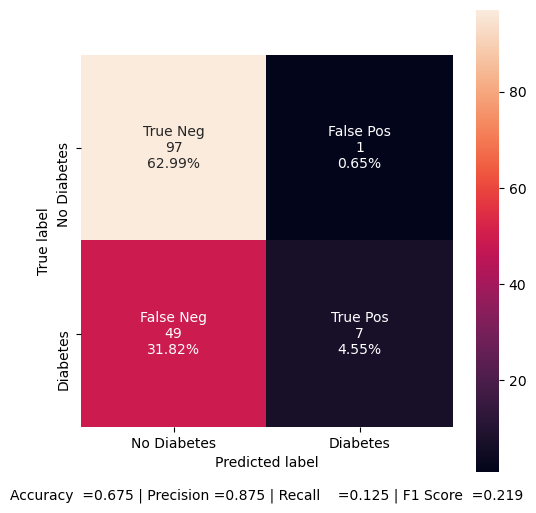
\includegraphics[height=200px]{../src_code/output/p1/unmodified/Confusion_matrix_[m:unmodified-C:0.1-K:linear-(1:5)]}} \,
\subfloat[2:5-Fold]{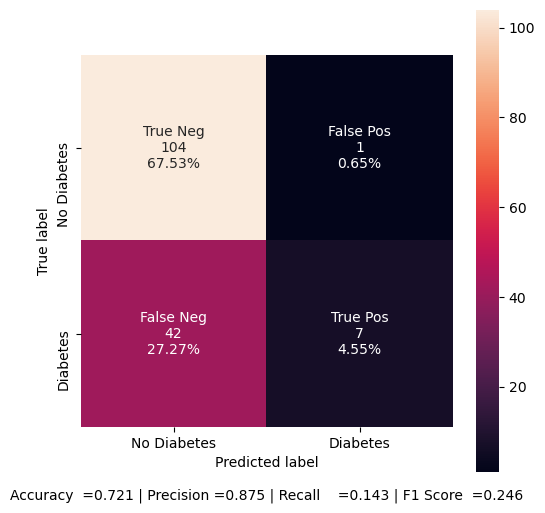
\includegraphics[height=200px]{../src_code/output/p1/unmodified/Confusion_matrix_[m:unmodified-C:0.1-K:linear-(2:5)]}} \,
\subfloat[3:5-Fold]{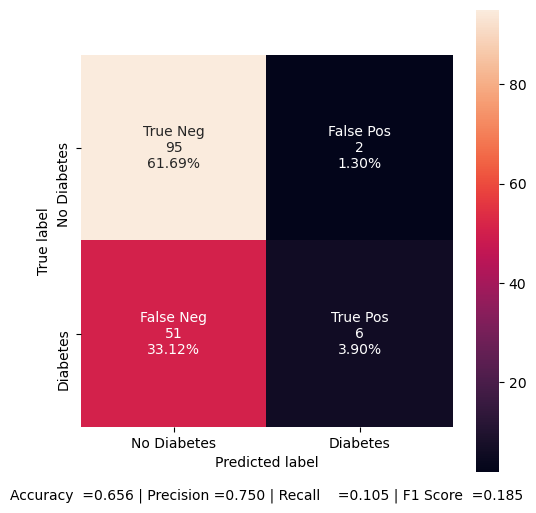
\includegraphics[height=200px]{../src_code/output/p1/unmodified/Confusion_matrix_[m:unmodified-C:0.1-K:linear-(3:5)]}} \,
\subfloat[4:5-Fold]{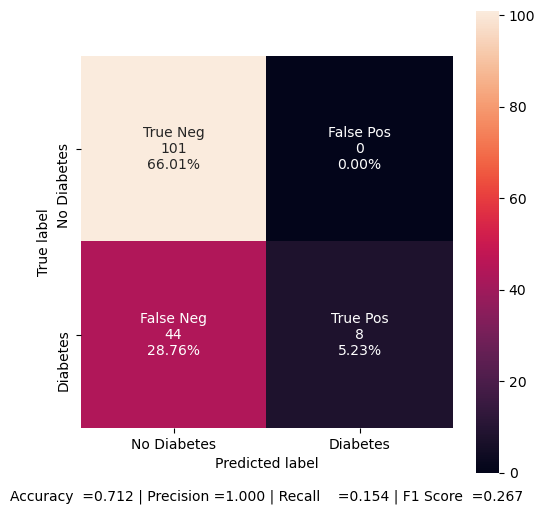
\includegraphics[height=200px]{../src_code/output/p1/unmodified/Confusion_matrix_[m:unmodified-C:0.1-K:linear-(4:5)]}} \,
\subfloat[5:5-Fold]{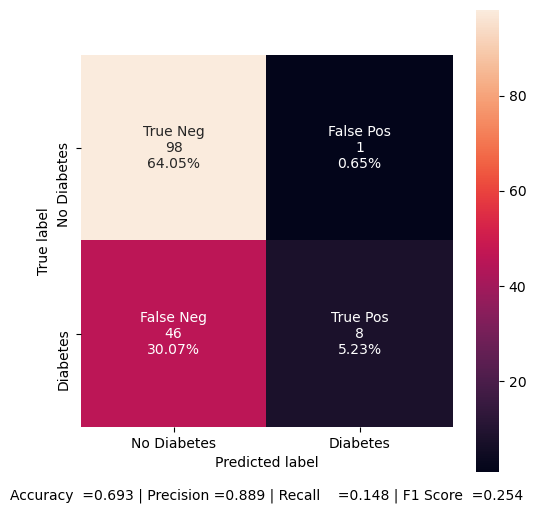
\includegraphics[height=200px]{../src_code/output/p1/unmodified/Confusion_matrix_[m:unmodified-C:0.1-K:linear-(5:5)]}} \,
\caption{Confusion Matrices for C:0.1 K:linear 5-fold}
\label{table:confusion:1}
\end{figure}


\begin{figure}[H]
\centering
\subfloat[1:5-Fold]{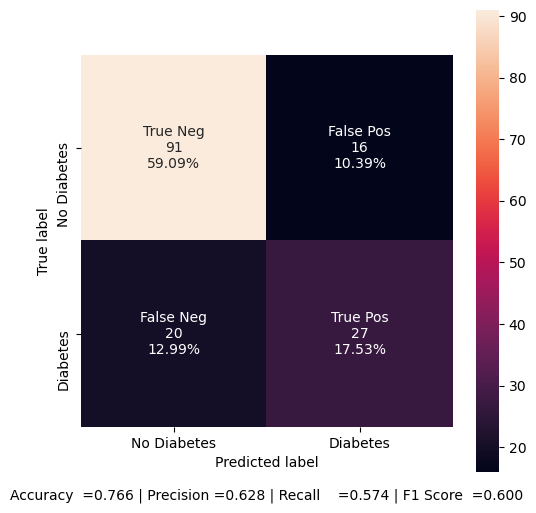
\includegraphics[height=200px]{../src_code/output/p1/unmodified/Confusion_matrix_[m:unmodified-C:0.1-K:poly-(1:5)]}} \,
\subfloat[2:5-Fold]{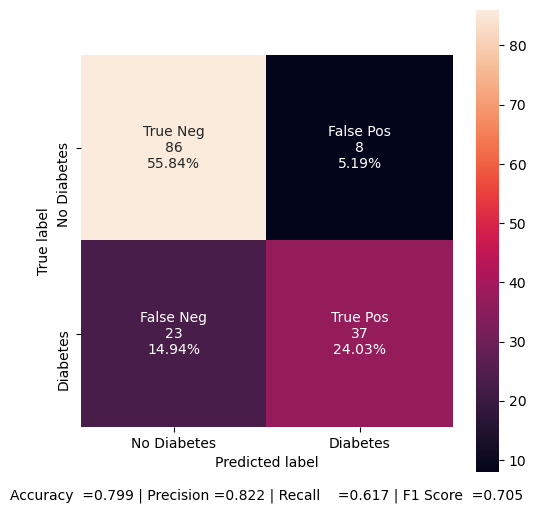
\includegraphics[height=200px]{../src_code/output/p1/unmodified/Confusion_matrix_[m:unmodified-C:0.1-K:poly-(2:5)]}} \,
\subfloat[3:5-Fold]{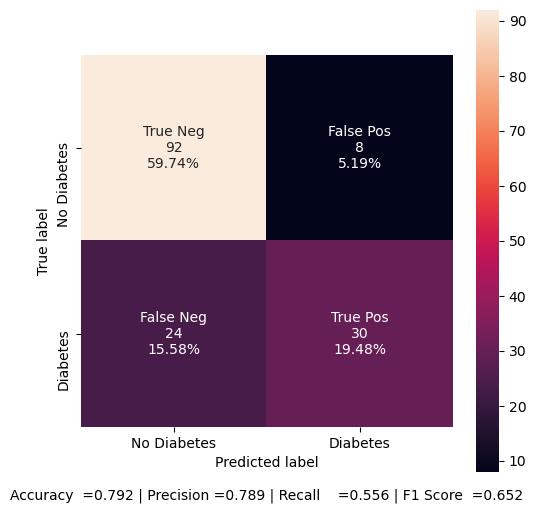
\includegraphics[height=200px]{../src_code/output/p1/unmodified/Confusion_matrix_[m:unmodified-C:0.1-K:poly-(3:5)]}} \,
\subfloat[4:5-Fold]{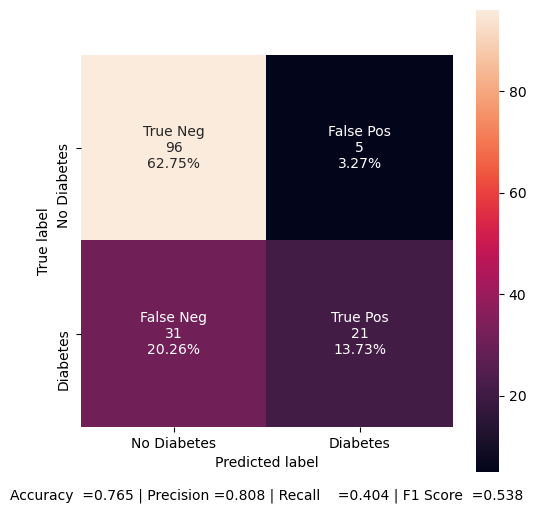
\includegraphics[height=200px]{../src_code/output/p1/unmodified/Confusion_matrix_[m:unmodified-C:0.1-K:poly-(4:5)]}} \,
\subfloat[5:5-Fold]{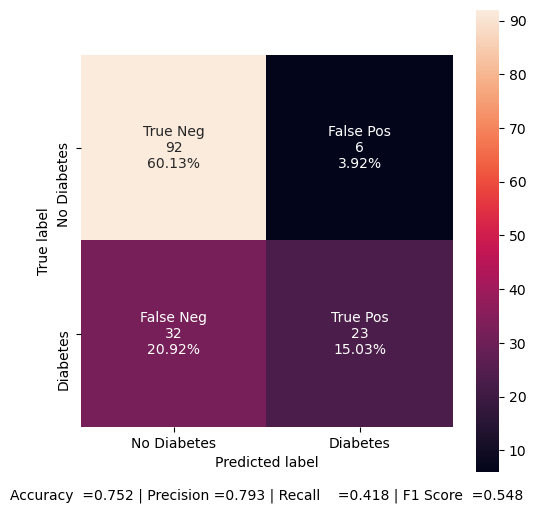
\includegraphics[height=200px]{../src_code/output/p1/unmodified/Confusion_matrix_[m:unmodified-C:0.1-K:poly-(5:5)]}} \,
\caption{Confusion Matrices for C:0.1 K:poly 5-fold}
\label{table:confusion:2}
\end{figure}


\begin{figure}[H]
\centering
\subfloat[1:5-Fold]{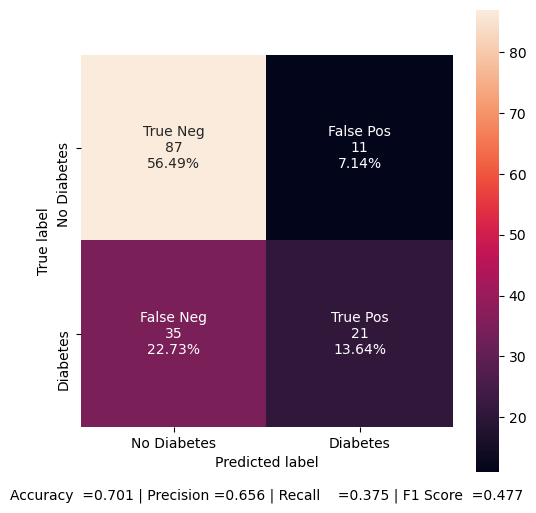
\includegraphics[height=200px]{../src_code/output/p1/unmodified/Confusion_matrix_[m:unmodified-C:0.1-K:rbf-(1:5)]}} \,
\subfloat[2:5-Fold]{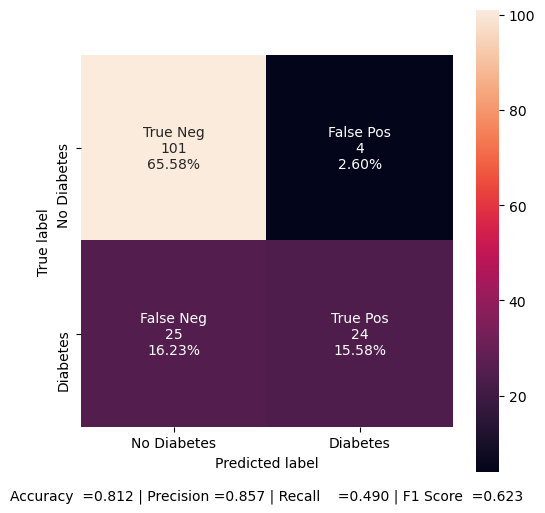
\includegraphics[height=200px]{../src_code/output/p1/unmodified/Confusion_matrix_[m:unmodified-C:0.1-K:rbf-(2:5)]}} \,
\subfloat[3:5-Fold]{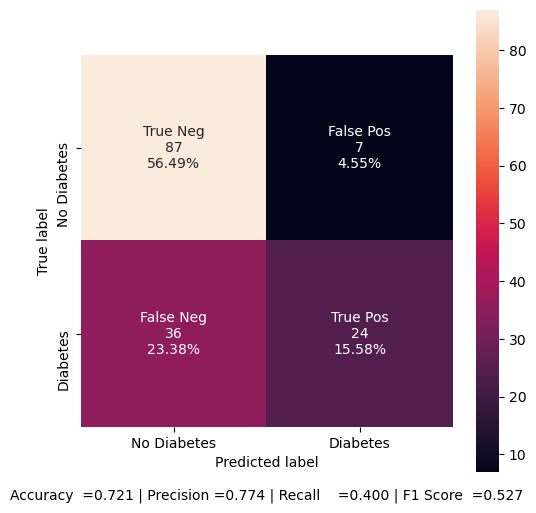
\includegraphics[height=200px]{../src_code/output/p1/unmodified/Confusion_matrix_[m:unmodified-C:0.1-K:rbf-(3:5)]}} \,
\subfloat[4:5-Fold]{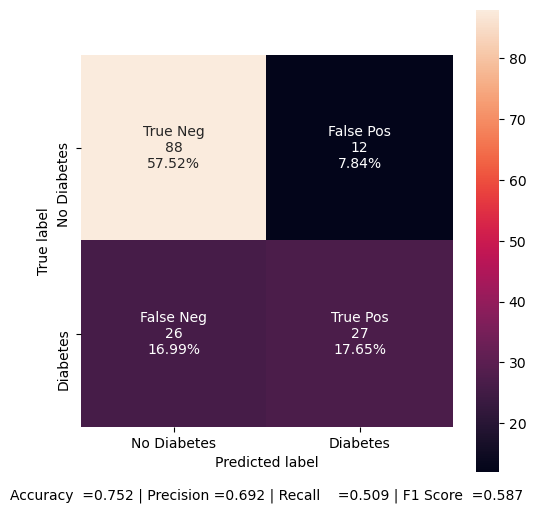
\includegraphics[height=200px]{../src_code/output/p1/unmodified/Confusion_matrix_[m:unmodified-C:0.1-K:rbf-(4:5)]}} \,
\subfloat[5:5-Fold]{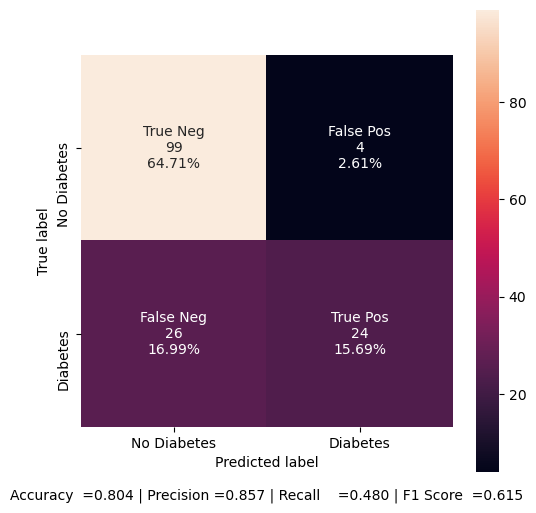
\includegraphics[height=200px]{../src_code/output/p1/unmodified/Confusion_matrix_[m:unmodified-C:0.1-K:rbf-(5:5)]}} \,
\caption{Confusion Matrices for C:0.1 K:rbf 5-fold}
\label{table:confusion:3}
\end{figure}


\begin{figure}[H]
\centering
\subfloat[1:5-Fold]{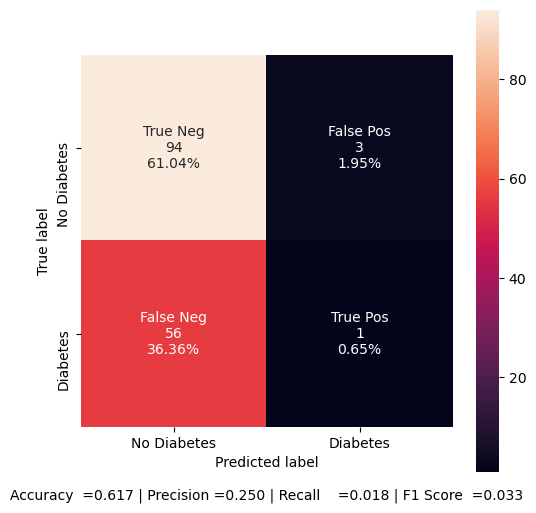
\includegraphics[height=200px]{../src_code/output/p1/unmodified/Confusion_matrix_[m:unmodified-C:0.1-K:sigmoid-(1:5)]}} \,
\subfloat[2:5-Fold]{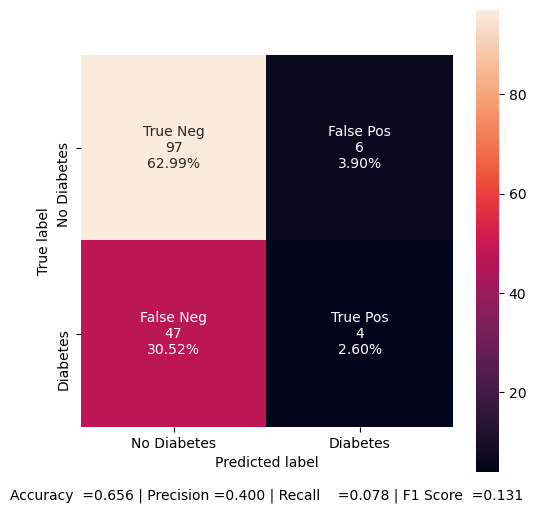
\includegraphics[height=200px]{../src_code/output/p1/unmodified/Confusion_matrix_[m:unmodified-C:0.1-K:sigmoid-(2:5)]}} \,
\subfloat[3:5-Fold]{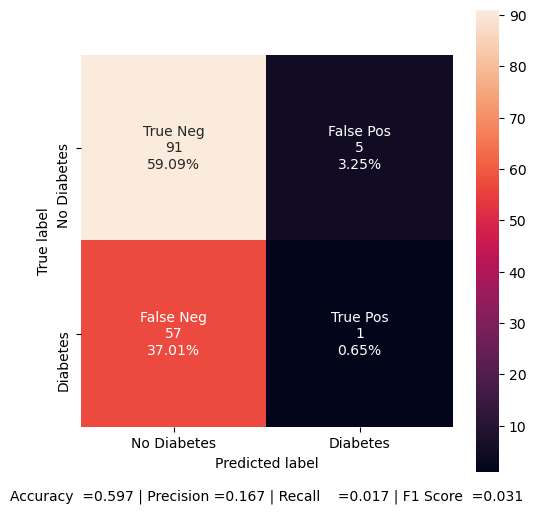
\includegraphics[height=200px]{../src_code/output/p1/unmodified/Confusion_matrix_[m:unmodified-C:0.1-K:sigmoid-(3:5)]}} \,
\subfloat[4:5-Fold]{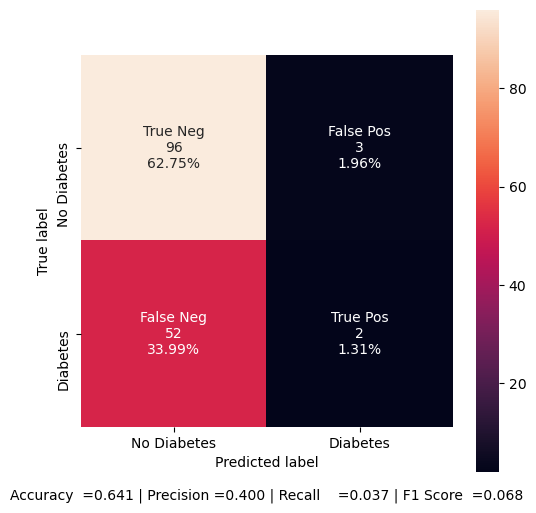
\includegraphics[height=200px]{../src_code/output/p1/unmodified/Confusion_matrix_[m:unmodified-C:0.1-K:sigmoid-(4:5)]}} \,
\subfloat[5:5-Fold]{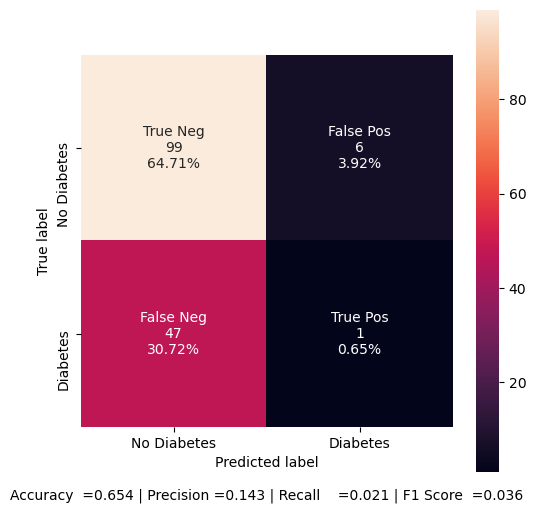
\includegraphics[height=200px]{../src_code/output/p1/unmodified/Confusion_matrix_[m:unmodified-C:0.1-K:sigmoid-(5:5)]}} \,
\caption{Confusion Matrices for C:0.1 K:sigmoid 5-fold}
\label{table:confusion:4}
\end{figure}


\begin{figure}[H]
\centering
\subfloat[1:5-Fold]{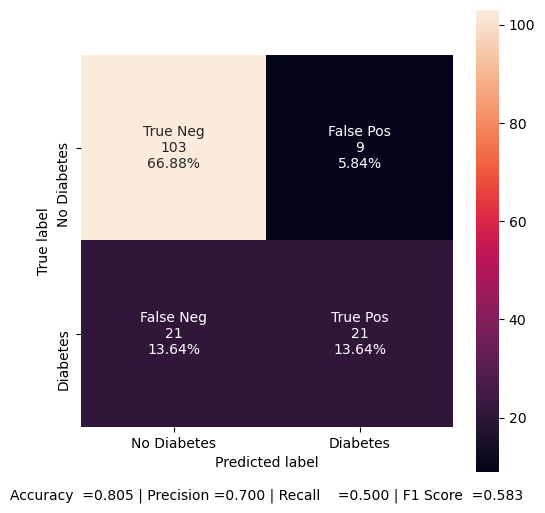
\includegraphics[height=200px]{../src_code/output/p1/unmodified/Confusion_matrix_[m:unmodified-C:1-K:linear-(1:5)]}} \,
\subfloat[2:5-Fold]{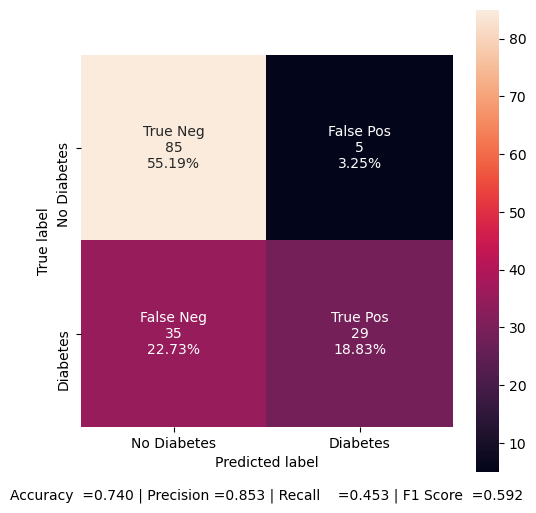
\includegraphics[height=200px]{../src_code/output/p1/unmodified/Confusion_matrix_[m:unmodified-C:1-K:linear-(2:5)]}} \,
\subfloat[3:5-Fold]{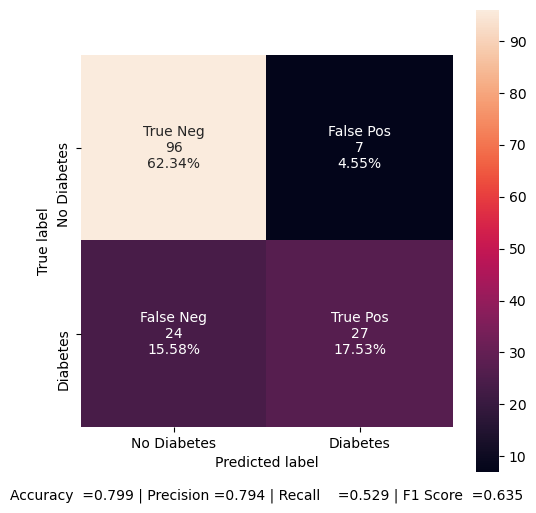
\includegraphics[height=200px]{../src_code/output/p1/unmodified/Confusion_matrix_[m:unmodified-C:1-K:linear-(3:5)]}} \,
\subfloat[4:5-Fold]{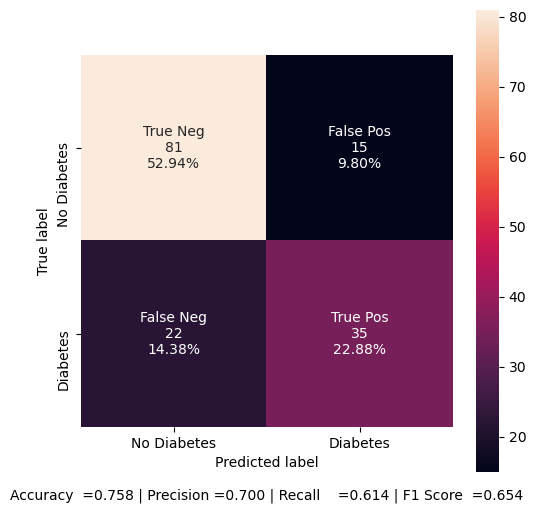
\includegraphics[height=200px]{../src_code/output/p1/unmodified/Confusion_matrix_[m:unmodified-C:1-K:linear-(4:5)]}} \,
\subfloat[5:5-Fold]{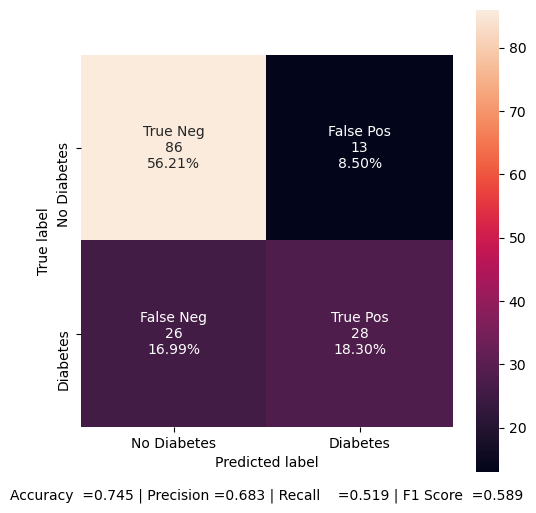
\includegraphics[height=200px]{../src_code/output/p1/unmodified/Confusion_matrix_[m:unmodified-C:1-K:linear-(5:5)]}} \,
\caption{Confusion Matrices for C:1 K:linear 5-fold}
\label{table:confusion:5}
\end{figure}


\begin{figure}[H]
\centering
\subfloat[1:5-Fold]{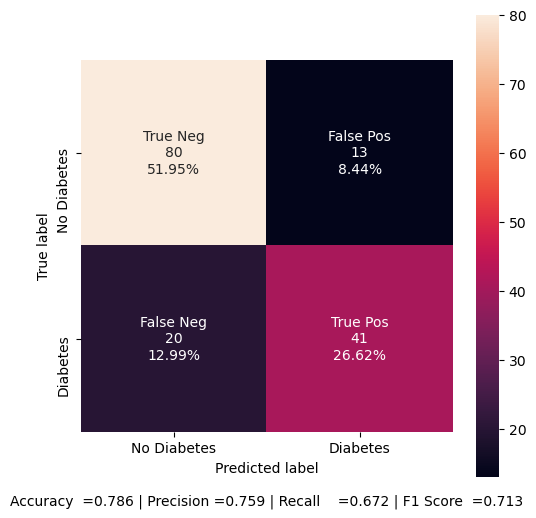
\includegraphics[height=200px]{../src_code/output/p1/unmodified/Confusion_matrix_[m:unmodified-C:1-K:poly-(1:5)]}} \,
\subfloat[2:5-Fold]{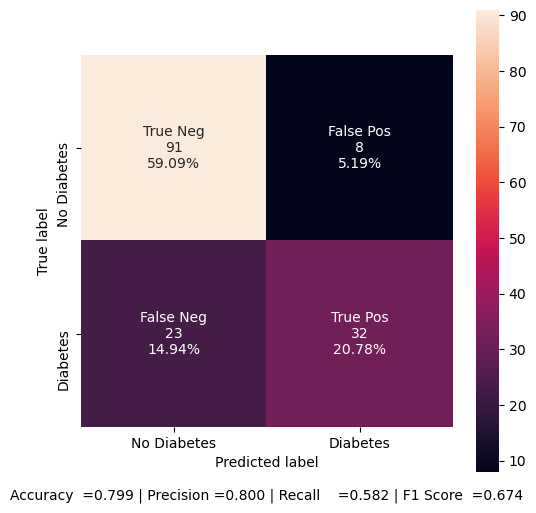
\includegraphics[height=200px]{../src_code/output/p1/unmodified/Confusion_matrix_[m:unmodified-C:1-K:poly-(2:5)]}} \,
\subfloat[3:5-Fold]{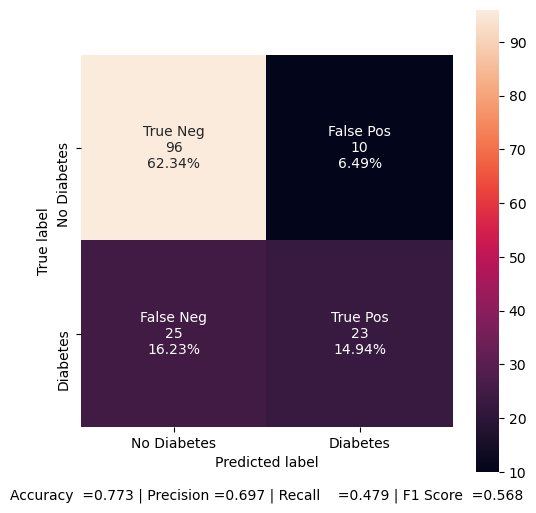
\includegraphics[height=200px]{../src_code/output/p1/unmodified/Confusion_matrix_[m:unmodified-C:1-K:poly-(3:5)]}} \,
\subfloat[4:5-Fold]{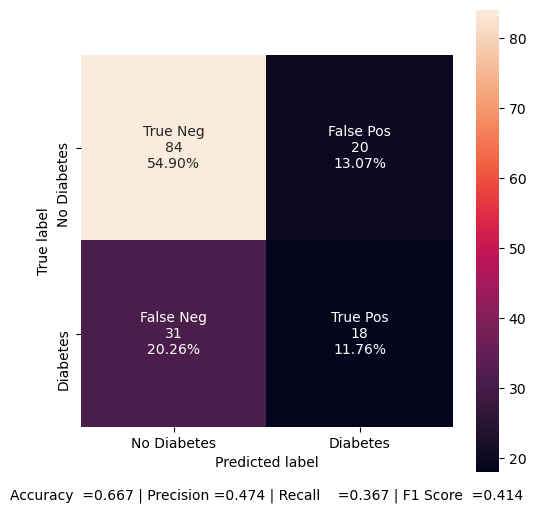
\includegraphics[height=200px]{../src_code/output/p1/unmodified/Confusion_matrix_[m:unmodified-C:1-K:poly-(4:5)]}} \,
\subfloat[5:5-Fold]{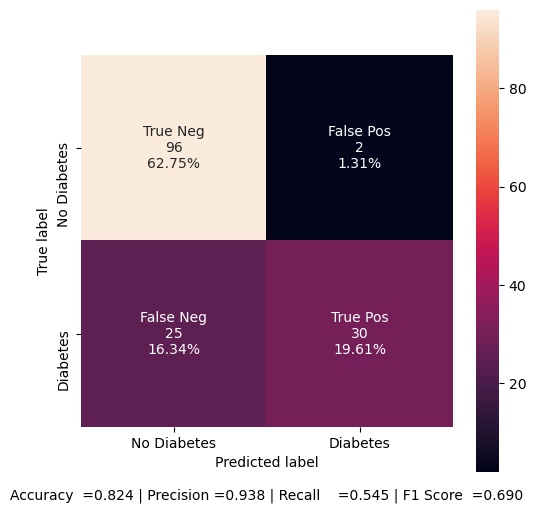
\includegraphics[height=200px]{../src_code/output/p1/unmodified/Confusion_matrix_[m:unmodified-C:1-K:poly-(5:5)]}} \,
\caption{Confusion Matrices for C:1 K:poly 5-fold}
\label{table:confusion:6}
\end{figure}


\begin{figure}[H]
\centering
\subfloat[1:5-Fold]{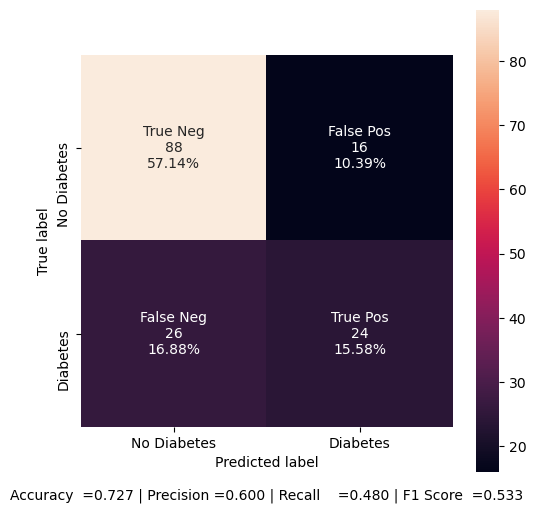
\includegraphics[height=200px]{../src_code/output/p1/unmodified/Confusion_matrix_[m:unmodified-C:1-K:rbf-(1:5)]}} \,
\subfloat[2:5-Fold]{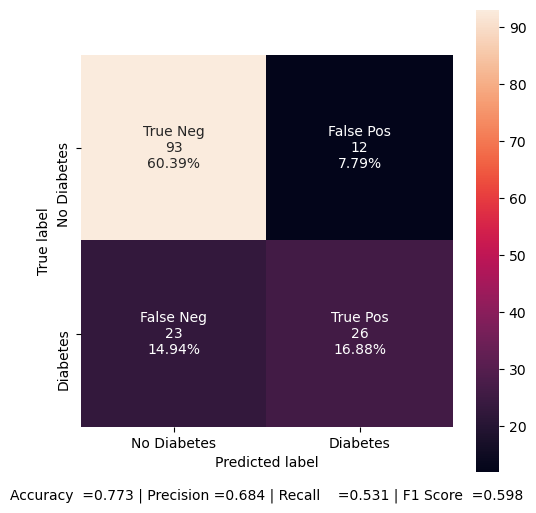
\includegraphics[height=200px]{../src_code/output/p1/unmodified/Confusion_matrix_[m:unmodified-C:1-K:rbf-(2:5)]}} \,
\subfloat[3:5-Fold]{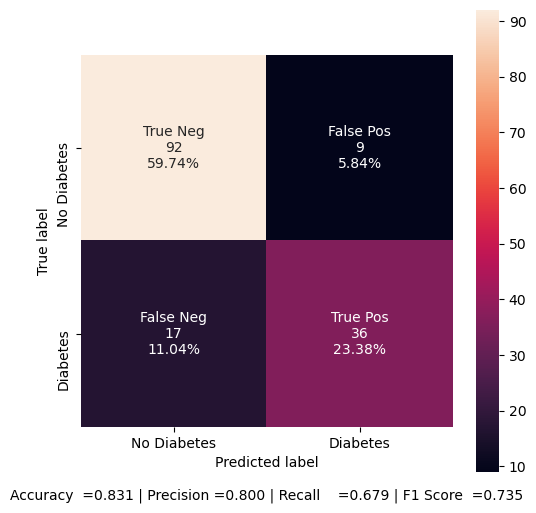
\includegraphics[height=200px]{../src_code/output/p1/unmodified/Confusion_matrix_[m:unmodified-C:1-K:rbf-(3:5)]}} \,
\subfloat[4:5-Fold]{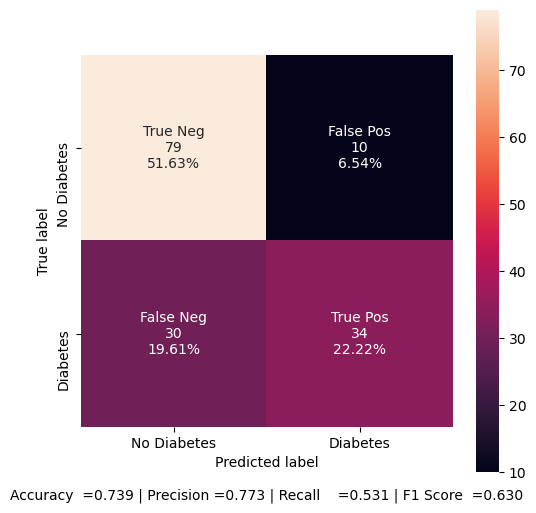
\includegraphics[height=200px]{../src_code/output/p1/unmodified/Confusion_matrix_[m:unmodified-C:1-K:rbf-(4:5)]}} \,
\subfloat[5:5-Fold]{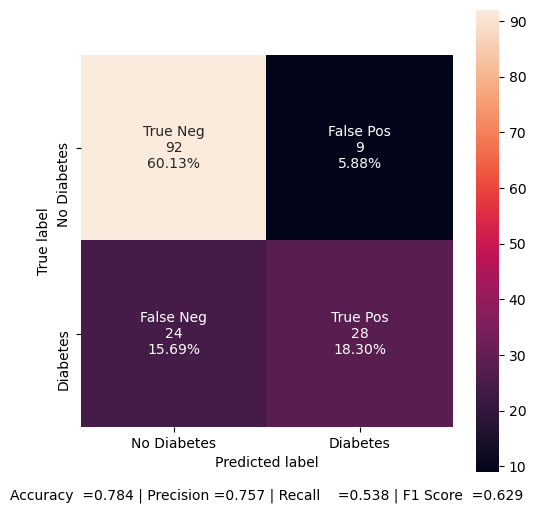
\includegraphics[height=200px]{../src_code/output/p1/unmodified/Confusion_matrix_[m:unmodified-C:1-K:rbf-(5:5)]}} \,
\caption{Confusion Matrices for C:1 K:rbf 5-fold}
\label{table:confusion:7}
\end{figure}


\begin{figure}[H]
\centering
\subfloat[1:5-Fold]{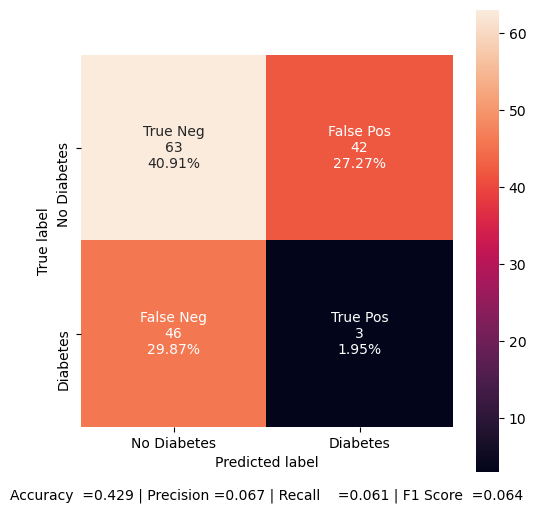
\includegraphics[height=200px]{../src_code/output/p1/unmodified/Confusion_matrix_[m:unmodified-C:1-K:sigmoid-(1:5)]}} \,
\subfloat[2:5-Fold]{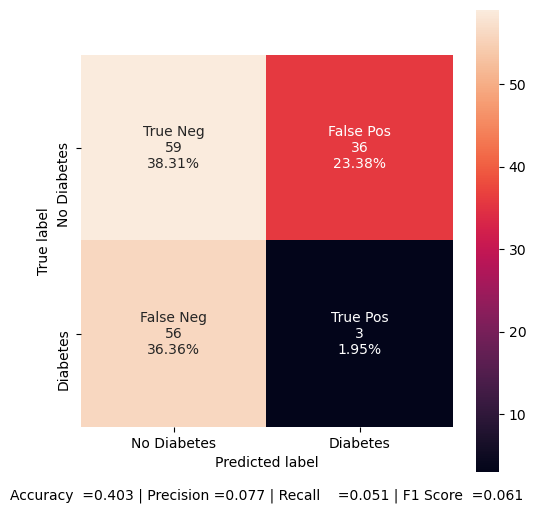
\includegraphics[height=200px]{../src_code/output/p1/unmodified/Confusion_matrix_[m:unmodified-C:1-K:sigmoid-(2:5)]}} \,
\subfloat[3:5-Fold]{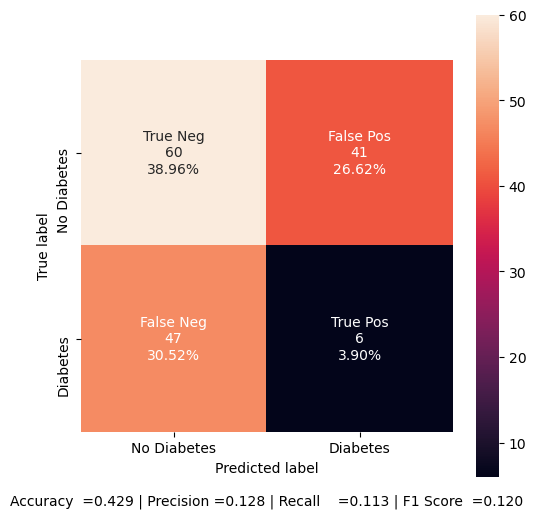
\includegraphics[height=200px]{../src_code/output/p1/unmodified/Confusion_matrix_[m:unmodified-C:1-K:sigmoid-(3:5)]}} \,
\subfloat[4:5-Fold]{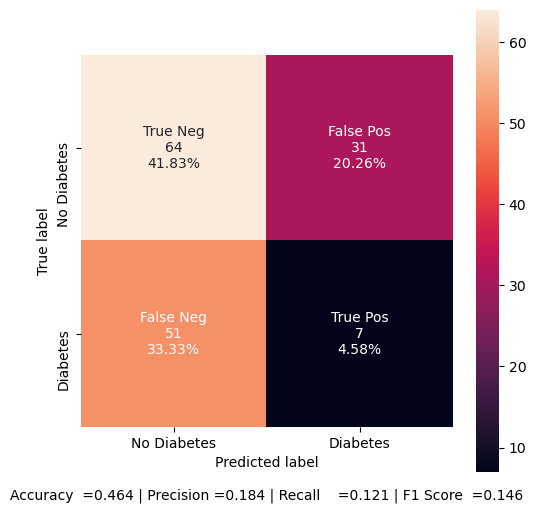
\includegraphics[height=200px]{../src_code/output/p1/unmodified/Confusion_matrix_[m:unmodified-C:1-K:sigmoid-(4:5)]}} \,
\subfloat[5:5-Fold]{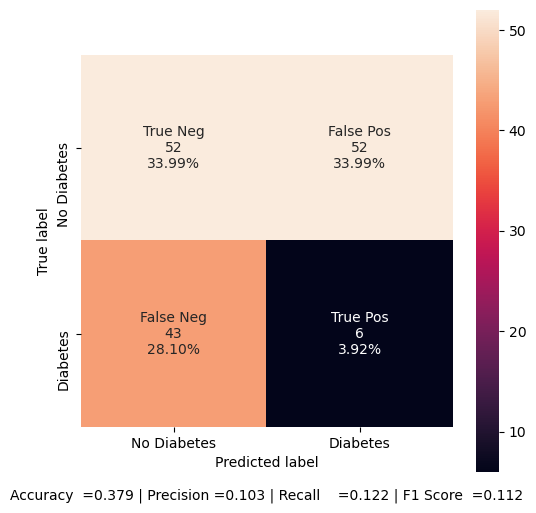
\includegraphics[height=200px]{../src_code/output/p1/unmodified/Confusion_matrix_[m:unmodified-C:1-K:sigmoid-(5:5)]}} \,
\caption{Confusion Matrices for C:1 K:sigmoid 5-fold}
\label{table:confusion:8}
\end{figure}


\begin{figure}[H]
\centering
\subfloat[1:5-Fold]{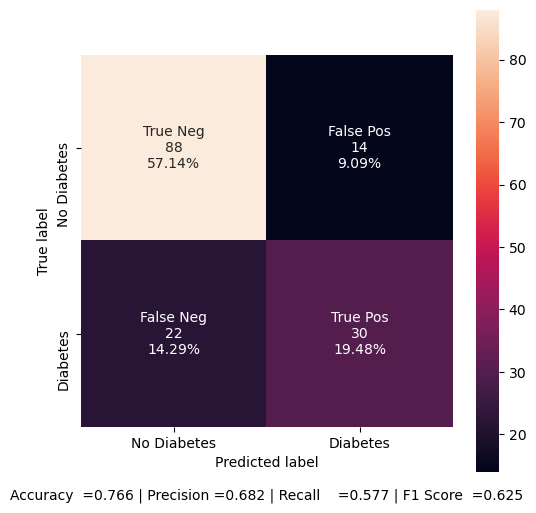
\includegraphics[height=200px]{../src_code/output/p1/unmodified/Confusion_matrix_[m:unmodified-C:5-K:linear-(1:5)]}} \,
\subfloat[2:5-Fold]{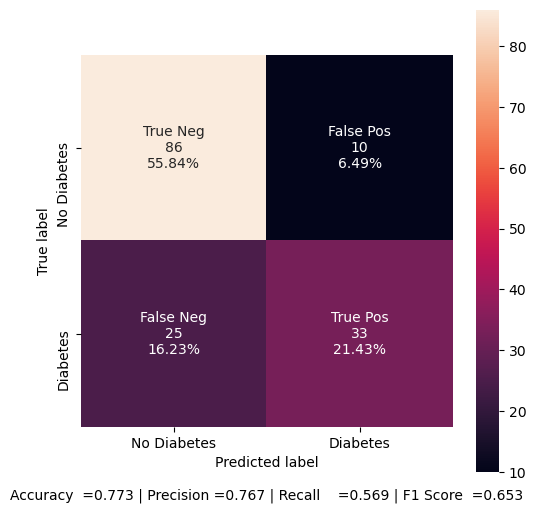
\includegraphics[height=200px]{../src_code/output/p1/unmodified/Confusion_matrix_[m:unmodified-C:5-K:linear-(2:5)]}} \,
\subfloat[3:5-Fold]{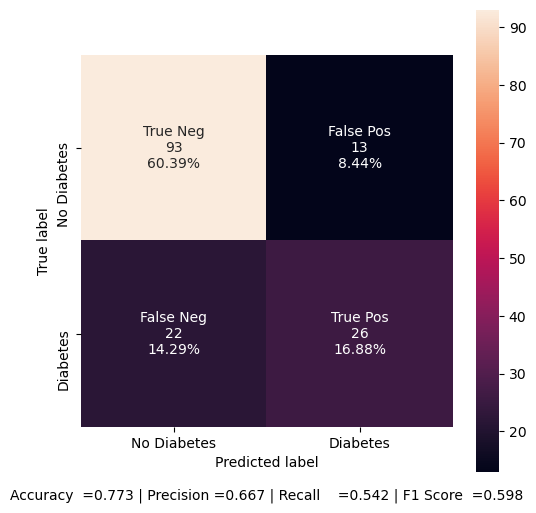
\includegraphics[height=200px]{../src_code/output/p1/unmodified/Confusion_matrix_[m:unmodified-C:5-K:linear-(3:5)]}} \,
\subfloat[4:5-Fold]{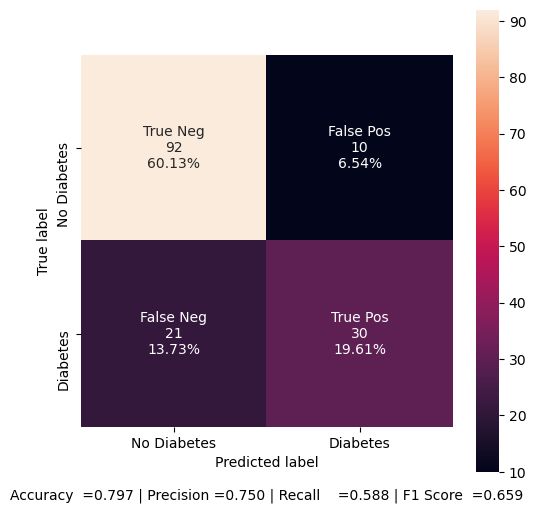
\includegraphics[height=200px]{../src_code/output/p1/unmodified/Confusion_matrix_[m:unmodified-C:5-K:linear-(4:5)]}} \,
\subfloat[5:5-Fold]{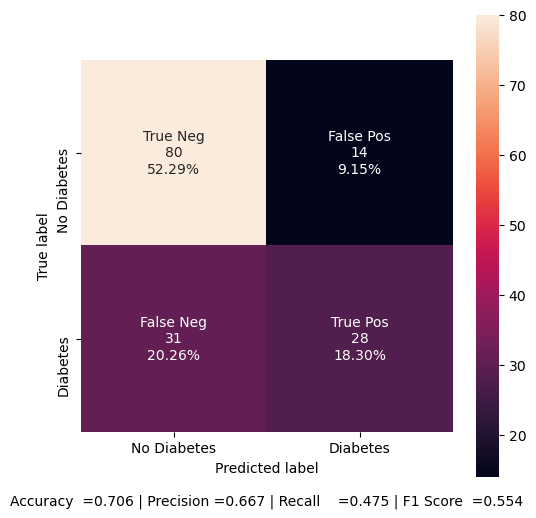
\includegraphics[height=200px]{../src_code/output/p1/unmodified/Confusion_matrix_[m:unmodified-C:5-K:linear-(5:5)]}} \,
\caption{Confusion Matrices for C:5 K:linear 5-fold}
\label{table:confusion:9}
\end{figure}


\begin{figure}[H]
\centering
\subfloat[1:5-Fold]{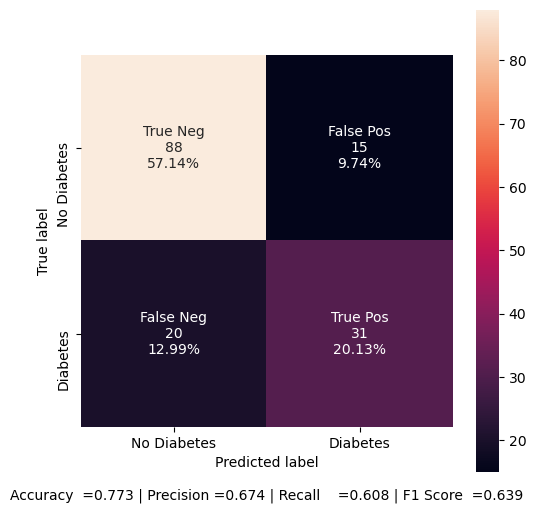
\includegraphics[height=200px]{../src_code/output/p1/unmodified/Confusion_matrix_[m:unmodified-C:5-K:poly-(1:5)]}} \,
\subfloat[2:5-Fold]{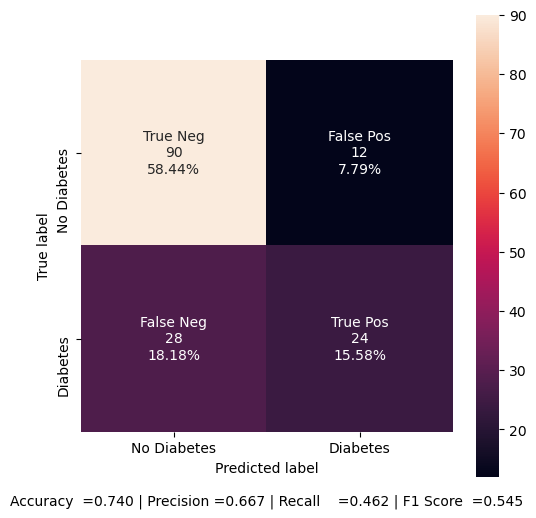
\includegraphics[height=200px]{../src_code/output/p1/unmodified/Confusion_matrix_[m:unmodified-C:5-K:poly-(2:5)]}} \,
\subfloat[3:5-Fold]{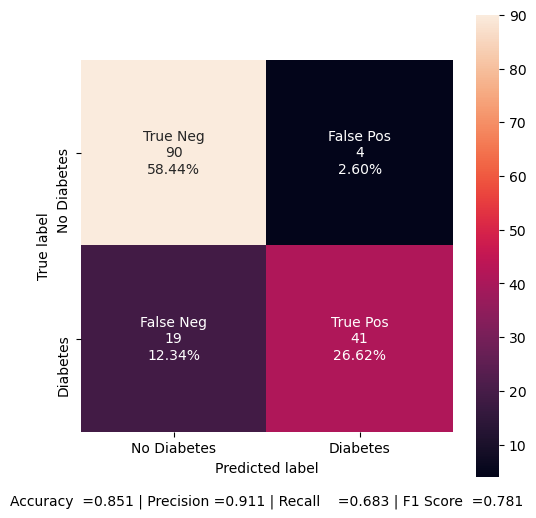
\includegraphics[height=200px]{../src_code/output/p1/unmodified/Confusion_matrix_[m:unmodified-C:5-K:poly-(3:5)]}} \,
\subfloat[4:5-Fold]{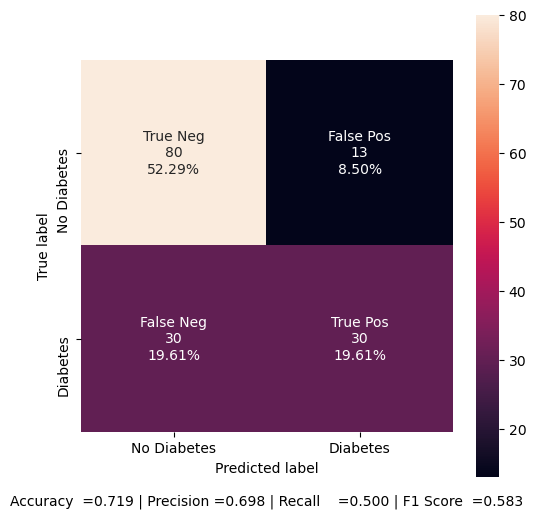
\includegraphics[height=200px]{../src_code/output/p1/unmodified/Confusion_matrix_[m:unmodified-C:5-K:poly-(4:5)]}} \,
\subfloat[5:5-Fold]{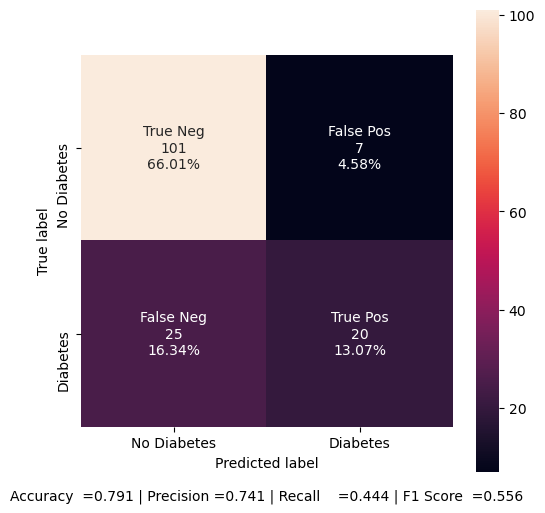
\includegraphics[height=200px]{../src_code/output/p1/unmodified/Confusion_matrix_[m:unmodified-C:5-K:poly-(5:5)]}} \,
\caption{Confusion Matrices for C:5 K:poly 5-fold}
\label{table:confusion:10}
\end{figure}


\begin{figure}[H]
\centering
\subfloat[1:5-Fold]{\includegraphics[height=200px]{../src_code/output/p1/unmodified/Confusion_matrix_[m:unmodified-C:5-K:rbf-(1:5)]}} \,
\subfloat[2:5-Fold]{\includegraphics[height=200px]{../src_code/output/p1/unmodified/Confusion_matrix_[m:unmodified-C:5-K:rbf-(2:5)]}} \,
\subfloat[3:5-Fold]{\includegraphics[height=200px]{../src_code/output/p1/unmodified/Confusion_matrix_[m:unmodified-C:5-K:rbf-(3:5)]}} \,
\subfloat[4:5-Fold]{\includegraphics[height=200px]{../src_code/output/p1/unmodified/Confusion_matrix_[m:unmodified-C:5-K:rbf-(4:5)]}} \,
\subfloat[5:5-Fold]{\includegraphics[height=200px]{../src_code/output/p1/unmodified/Confusion_matrix_[m:unmodified-C:5-K:rbf-(5:5)]}} \,
\caption{Confusion Matrices for C:5 K:rbf 5-fold}
\label{table:confusion:11}
\end{figure}


\begin{figure}[H]
\centering
\subfloat[1:5-Fold]{\includegraphics[height=200px]{../src_code/output/p1/unmodified/Confusion_matrix_[m:unmodified-C:5-K:sigmoid-(1:5)]}} \,
\subfloat[2:5-Fold]{\includegraphics[height=200px]{../src_code/output/p1/unmodified/Confusion_matrix_[m:unmodified-C:5-K:sigmoid-(2:5)]}} \,
\subfloat[3:5-Fold]{\includegraphics[height=200px]{../src_code/output/p1/unmodified/Confusion_matrix_[m:unmodified-C:5-K:sigmoid-(3:5)]}} \,
\subfloat[4:5-Fold]{\includegraphics[height=200px]{../src_code/output/p1/unmodified/Confusion_matrix_[m:unmodified-C:5-K:sigmoid-(4:5)]}} \,
\subfloat[5:5-Fold]{\includegraphics[height=200px]{../src_code/output/p1/unmodified/Confusion_matrix_[m:unmodified-C:5-K:sigmoid-(5:5)]}} \,
\caption{Confusion Matrices for C:5 K:sigmoid 5-fold}
\label{table:confusion:12}
\end{figure}


\begin{figure}[H]
\centering
\subfloat[1:5-Fold]{\includegraphics[height=200px]{../src_code/output/p1/unmodified/Confusion_matrix_[m:unmodified-C:10-K:linear-(1:5)]}} \,
\subfloat[2:5-Fold]{\includegraphics[height=200px]{../src_code/output/p1/unmodified/Confusion_matrix_[m:unmodified-C:10-K:linear-(2:5)]}} \,
\subfloat[3:5-Fold]{\includegraphics[height=200px]{../src_code/output/p1/unmodified/Confusion_matrix_[m:unmodified-C:10-K:linear-(3:5)]}} \,
\subfloat[4:5-Fold]{\includegraphics[height=200px]{../src_code/output/p1/unmodified/Confusion_matrix_[m:unmodified-C:10-K:linear-(4:5)]}} \,
\subfloat[5:5-Fold]{\includegraphics[height=200px]{../src_code/output/p1/unmodified/Confusion_matrix_[m:unmodified-C:10-K:linear-(5:5)]}} \,
\caption{Confusion Matrices for C:10 K:linear 5-fold}
\label{table:confusion:13}
\end{figure}


\begin{figure}[H]
\centering
\subfloat[1:5-Fold]{\includegraphics[height=200px]{../src_code/output/p1/unmodified/Confusion_matrix_[m:unmodified-C:10-K:poly-(1:5)]}} \,
\subfloat[2:5-Fold]{\includegraphics[height=200px]{../src_code/output/p1/unmodified/Confusion_matrix_[m:unmodified-C:10-K:poly-(2:5)]}} \,
\subfloat[3:5-Fold]{\includegraphics[height=200px]{../src_code/output/p1/unmodified/Confusion_matrix_[m:unmodified-C:10-K:poly-(3:5)]}} \,
\subfloat[4:5-Fold]{\includegraphics[height=200px]{../src_code/output/p1/unmodified/Confusion_matrix_[m:unmodified-C:10-K:poly-(4:5)]}} \,
\subfloat[5:5-Fold]{\includegraphics[height=200px]{../src_code/output/p1/unmodified/Confusion_matrix_[m:unmodified-C:10-K:poly-(5:5)]}} \,
\caption{Confusion Matrices for C:10 K:poly 5-fold}
\label{table:confusion:14}
\end{figure}


\begin{figure}[H]
\centering
\subfloat[1:5-Fold]{\includegraphics[height=200px]{../src_code/output/p1/unmodified/Confusion_matrix_[m:unmodified-C:10-K:rbf-(1:5)]}} \,
\subfloat[2:5-Fold]{\includegraphics[height=200px]{../src_code/output/p1/unmodified/Confusion_matrix_[m:unmodified-C:10-K:rbf-(2:5)]}} \,
\subfloat[3:5-Fold]{\includegraphics[height=200px]{../src_code/output/p1/unmodified/Confusion_matrix_[m:unmodified-C:10-K:rbf-(3:5)]}} \,
\subfloat[4:5-Fold]{\includegraphics[height=200px]{../src_code/output/p1/unmodified/Confusion_matrix_[m:unmodified-C:10-K:rbf-(4:5)]}} \,
\subfloat[5:5-Fold]{\includegraphics[height=200px]{../src_code/output/p1/unmodified/Confusion_matrix_[m:unmodified-C:10-K:rbf-(5:5)]}} \,
\caption{Confusion Matrices for C:10 K:rbf 5-fold}
\label{table:confusion:15}
\end{figure}


\begin{figure}[H]
\centering
\subfloat[1:5-Fold]{\includegraphics[height=200px]{../src_code/output/p1/unmodified/Confusion_matrix_[m:unmodified-C:10-K:sigmoid-(1:5)]}} \,
\subfloat[2:5-Fold]{\includegraphics[height=200px]{../src_code/output/p1/unmodified/Confusion_matrix_[m:unmodified-C:10-K:sigmoid-(2:5)]}} \,
\subfloat[3:5-Fold]{\includegraphics[height=200px]{../src_code/output/p1/unmodified/Confusion_matrix_[m:unmodified-C:10-K:sigmoid-(3:5)]}} \,
\subfloat[4:5-Fold]{\includegraphics[height=200px]{../src_code/output/p1/unmodified/Confusion_matrix_[m:unmodified-C:10-K:sigmoid-(4:5)]}} \,
\subfloat[5:5-Fold]{\includegraphics[height=200px]{../src_code/output/p1/unmodified/Confusion_matrix_[m:unmodified-C:10-K:sigmoid-(5:5)]}} \,
\caption{Confusion Matrices for C:10 K:sigmoid 5-fold}
\label{table:confusion:16}
\end{figure}

\subsection{(b): Various performance measure (15 marks)}
% 2. (15 marks) Write the various performance measure in terms of Accuracy, Precision, Recall, and F1 Measure. Which performance measure is most important in this problem? Why?

The performance measure is calculated along with confusion matrices (full implementation can be found in \Cref{code:jx_lib}):
\lstinputlisting[language=python, caption=SVM Performance Measure, label=code:p1:performance, linerange={90-98}]{../src_code/jx_lib.py}

The average, best, and worst performance measures out of 5-fold cross-validation in terms of Accuracy, Precision, Recall, and F1 Measure are summarized in \Cref{table:performance-grid:avg}, \Cref{table:performance-grid:best}, and \Cref{table:performance-grid:worst} respectively.

The recall measure is the most important in this problem, since we want to eliminate percent of false negative to ensure it is not missing any people who are indeed having diabetes. In another word, we need to maximizing percent of true positive over sum of true positive and false positive, which is the recall performance measure. In addition, the worst performance measure of the recall out of 5-Fold cross-validation shall be also considered when choosing the model, since we would always ensure the worst possible performance of the model. 

\begin{figure}[H]
\centering
	\includegraphics[height=400px]{../src_code/output/p1/unmodified/Summary_unmodified_average}
	\caption{Average performance grid matrices for all 16 combinations}
	\label{table:performance-grid:avg}
\end{figure}

\begin{figure}[H]
\centering
	\includegraphics[height=400px]{../src_code/output/p1/unmodified/Summary_unmodified_best}
	\caption{Best performance grid matrices for all 16 combinations}
	\label{table:performance-grid:best}
\end{figure}

\begin{figure}[H]
\centering
	\includegraphics[height=400px]{../src_code/output/p1/unmodified/Summary_unmodified_worst}
	\caption{Worst performance grid matrices for all 16 combinations}
	\label{table:performance-grid:worst}
\end{figure}

\clearpage
\subsection{Extra Self-studies*}
We may wonder how do we improve the accuracy? The main strategy is about pre-processing to manipulate the sample data, such as balancing the training dataset, removing outliers, and ensuring the dataset is uncorrelated. For the sake of fun, we start with the study of dataset distribution.

As we may discover in \Cref{fig:p1:distributions}, the dataset appeared to be unbalanced with positive and negative labels, hence we shall balance them by concatenating repetitive dataset in the positive samples.
\begin{figure}[H]
\centering
	\subfloat[Original dataset]{\includegraphics[height=200px]{../src_code/output/p1/balance/Pie_balance_Original_data.png}}\,
	\subfloat[Balanced dataset]{\includegraphics[height=200px]{../src_code/output/p1/balance/Pie_balance_Balanced_data.png}}
	\caption{Dataset label distributions}
	\label{fig:p1:distributions}
\end{figure}

Let's plot their new performance grids below. As we may find from \Cref{table:balanced:performance-grid:avg} - \Cref{table:balanced:performance-grid:worst}, the overall worst cases are much better than the unbalanced dataset. However, we do see the recall measures may differ depends on the combinations. Hence, further data manipulation is needed, such as the feature reduction is needed. Since the SVM is quite sensitive to outliers, an outlier filter should also be applied to the dataset to increase the performance of the recall measure.

\begin{figure}[H]
\centering
	\includegraphics[height=400px]{../src_code/output/p1/balance/Summary_balance_average}
	\caption{Average performance grid matrices for all 16 combinations (Balanced)}
	\label{table:balanced:performance-grid:avg}
\end{figure}

\begin{figure}[H]
\centering
	\includegraphics[height=400px]{../src_code/output/p1/balance/Summary_balance_best}
	\caption{Best performance grid matrices for all 16 combinations (Balanced)}
	\label{table:balanced:performance-grid:best}
\end{figure}

\begin{figure}[H]
\centering
	\includegraphics[height=400px]{../src_code/output/p1/balance/Summary_balance_worst}
	\caption{Worst performance grid matrices for all 16 combinations (Balanced)}
	\label{table:balanced:performance-grid:worst}
\end{figure}



%%%%%%%%%%%%%%%%
%%%%% Ex 2 %%%%%
%%%%%%%%%%%%%%%%
\newpage
\section{Problem 2: Kohonen Self Organizng Map: Unsupervised Learning [\Cref{code:p2}]}
%{
%	We need to design a Kohonen self organizing map (SOM), which gives as an output some shades of color mapped over 100 by 100 grid of neurones. The idea is to cluster colors of the same shade in the same neighborhood using 3D to 2D representation of colors. The training input of the SOM are 24 colors (use shades of red, green, blue, with some yellow, teal and pink) which you can chose from the "RGB Color Table: Basic Colors" section of this page: http://www.rapidtables.com/web/color/RGB_Color.htm
%	
%	Using a time varying learning rate
%	
%	a (k) = a (0)exp(-k /T)
%	
%	where k is the current training
%	
%	epoch (starts with epoch 0), 𝛼 ( 0 ) = 0.8 , and T is the Total number of training epochs equal to 600. Note that the epoch training involves all twenty four input samples for the 24 chosen colors to the network (hint: calibrate the color codes to values between 0 and 1, instead of being between 0 and 255). The initial weights linking to all 10,000 output nodes are randomized. Basically each node has an RGB color of three random values between ( 0 and 255, which should be normalized to between 0 and 1 in the same way we calibrate the training data as discussed earlier)
% ..... (see pdf)
%}
\subsection{Implementation (Matrix Formulation and Optimization)}
In order to optimize the performance and utilize the gpu performance, the update function is modelled and implemented in matrix forms, and any constant is being pre-computed in each iteration, as shown in \Cref{code:p2:opt}. 
\lstinputlisting[language=python, caption=KSOM Core Update in Matrix Formulation, label=code:p2:opt, firstline=61, lastline=83]{../src_code/as2_p2.py}

The final outcome is outstanding, where it only takes 37.8 seconds to compute, in comparison to the double for loop form, which takes minutes and even hours to compute.
\begin{lstlisting}[style=mystyle:output]
[Running] python -u "/Users/jaku/JX-Platform/Github/UW__4B_Individual_Works/ECE_457B/A2/src_code/as2_p2.py"
ic| normRGB.shape: (24, 3)
Epoch Number: 1
Epoch Number: 20
Epoch Number: 40
Epoch Number: 100
Epoch Number: 600
Epoch Number: 1
Epoch Number: 20
Epoch Number: 40
Epoch Number: 100
Epoch Number: 600
Epoch Number: 1
Epoch Number: 20
Epoch Number: 40
Epoch Number: 100
Epoch Number: 600

[Done] exited with code=0 in 37.838 seconds
\end{lstlisting}

\subsection{(a): SOM Grids Result (25 marks)}
% a) (25 marks) Basically, and after training, we need to have as the output of the SOM colors something similar to the picture below, where similar colors cluster around each other’s:
% Generate, a figure of the original SOM grid (randomly selected) followed by figures of the SOM grid after 20, 40, 100, 600 epochs for various values of s 0 =10, 40,70 .
A random SOM grid is generated initially as seen in \Cref{fig:p2:orig}
\begin{figure}[H]
	\center
	\includegraphics[height=120px]{../src_code/output/p2/w_0}
	\caption{Original SOM grid (random colors)}
	\label{fig:p2:orig}
\end{figure}

A set of 24 colors are randomly selected from the HSV wheels as shown in \Cref{fig:p2:colorbar}
\begin{figure}[H]
	\center
	\includegraphics[height=50px]{../src_code/output/p2/color_bar}
	\caption{24 randomly selected colors (from HSV wheel to RGB)}
	\label{fig:p2:colorbar}
\end{figure}

The resultant SOM grids are summarized in \Cref{table:som} below:
\begin{longtable}{p{1cm} p{4.5cm} p{4.5cm} p{4.5cm}} \hline
	%% Header
	& \textbf{$\sigma_0 = 10$} & \textbf{$\sigma_0 = 40$} & \textbf{$\sigma_0 = 70$}
	\\ \hline
	%% Content
	Epochs = 1 	
		& \raisebox{-120px}{\includegraphics[height=120px]{../src_code/output/p2/[s=10]_w_1}} 
		& \raisebox{-120px}{\includegraphics[height=120px]{../src_code/output/p2/[s=40]_w_1}} 
		& \raisebox{-120px}{\includegraphics[height=120px]{../src_code/output/p2/[s=70]_w_1}} 
	\\ \hline
	Epochs = 20 	
		& \raisebox{-120px}{\includegraphics[height=120px]{../src_code/output/p2/[s=10]_w_20}} 
		& \raisebox{-120px}{\includegraphics[height=120px]{../src_code/output/p2/[s=40]_w_20}} 
		& \raisebox{-120px}{\includegraphics[height=120px]{../src_code/output/p2/[s=70]_w_20}} 
	\\ \hline
	Epochs = 40 	
		& \raisebox{-120px}{\includegraphics[height=120px]{../src_code/output/p2/[s=10]_w_40}} 
		& \raisebox{-120px}{\includegraphics[height=120px]{../src_code/output/p2/[s=40]_w_40}} 
		& \raisebox{-120px}{\includegraphics[height=120px]{../src_code/output/p2/[s=70]_w_40}} 
	\\ \hline
	Epochs = 100 	
		& \raisebox{-120px}{\includegraphics[height=120px]{../src_code/output/p2/[s=10]_w_100}} 
		& \raisebox{-120px}{\includegraphics[height=120px]{../src_code/output/p2/[s=40]_w_100}} 
		& \raisebox{-120px}{\includegraphics[height=120px]{../src_code/output/p2/[s=70]_w_100}} 
	\\ \hline
	Epochs = 600 	
		& \raisebox{-120px}{\includegraphics[height=120px]{../src_code/output/p2/[s=10]_w_600}} 
		& \raisebox{-120px}{\includegraphics[height=120px]{../src_code/output/p2/[s=40]_w_600}} 
		& \raisebox{-120px}{\includegraphics[height=120px]{../src_code/output/p2/[s=70]_w_600}} 
	\\ \hline
	Epochs = 1000 	
		& \raisebox{-120px}{\includegraphics[height=120px]{../src_code/output/p2/[s=10]_w_1000}} 
		& \raisebox{-120px}{\includegraphics[height=120px]{../src_code/output/p2/[s=40]_w_1000}} 
		& \raisebox{-120px}{\includegraphics[height=120px]{../src_code/output/p2/[s=70]_w_1000}} 
	\\ \hline
	Epochs = 1500	
		& \raisebox{-120px}{\includegraphics[height=120px]{../src_code/output/p2/[s=10]_w_1500}} 
		& \raisebox{-120px}{\includegraphics[height=120px]{../src_code/output/p2/[s=40]_w_1500}} 
		& \raisebox{-120px}{\includegraphics[height=120px]{../src_code/output/p2/[s=70]_w_1500}} 
	\\ \hline
	Epochs = 2000 	
		& \raisebox{-120px}{\includegraphics[height=120px]{../src_code/output/p2/[s=10]_w_2000}} 
		& \raisebox{-120px}{\includegraphics[height=120px]{../src_code/output/p2/[s=40]_w_2000}} 
		& \raisebox{-120px}{\includegraphics[height=120px]{../src_code/output/p2/[s=70]_w_2000}} 
	\\ \hline
	\caption{SOM grid summary table for various $\sigma_0$ at different epochs} % needs to go inside longtable environment
	\label{table:som}
\end{longtable}


\subsection{(b): Conclusions (5 marks)}
% b) (5 marks) In light of the above simulations, draw your conclusions?
%. https://www.cs.hmc.edu/~kpang/nn/som.html
The above implementation utilizes an adaptive neighboring, as the neighborhood variance decreases overtime, resulting a smaller neighbor size. This is done to help neurons initially adjust their weights to roughly where they want to be then allow them to converge without being dramatically influenced by "winning" neurons that are far away. In another world, the early stage is the self-organizing or re-ordering phase, and the later stage is fine tuning phase to make the grid coverge. 

From the above simulation as tabulated in \Cref{table:som}, we may find the SOM is capable to cluster progressively based on the given training dataset without any supervision. The initial variance of the topological neighborhood size ($\sigma_0$) affects the convergence rate and granularity of the SOM grid. A smaller initial variance may potentially not utilize all the parameters on the map (as seen at "epochs=1"), resulting an unstable grid initially. But it converges to the final stability much faster, and provides a much granular-looking SOM grid with sharp boundaries in result of a smaller neighborhood size, as shown by the column for $\sigma_0 = 10$. A larger initial variance converges much slower to the final stability, but provides a more even and generalized SOM grid with blended margins, as shown by the column for $\sigma_0 = 70$. We may find the medium variance of $\sigma_0 = 40$ between the two extremes provided the best outcome of the SOM grid, as it quickly reaches equilibrium quick enough without loosing any color varieties, and provides a finer final SOM grid that is more generalized. 

In short, the magical SOM performance depends on the initial neighbouring size for the adaptive neighborhood function (Gaussian specifically in our case). The neighborhood size essentially determines number of neurons being utilized, which determines the granurality or the scale of the resulting model. A smaller variance provides a less generalized model but more accurate boundaries, as it overfits with a sharp decision boundaries. A larger variance provides a more generalized model, but converges to the final equilibrium much slower and provides less accuracy. Its two contradictory behaviours, where we either gain generalization or accuracy and loose the other as the trade of.


%%%%%%%%%%%%%%%%
%%%%% Ex 3 %%%%%
%%%%%%%%%%%%%%%%
\newpage
\section{Problem 3: MLP vs Deep Learning Based CNN [\Cref{code:p3}]}

%{
%	Using your preferred deep learning library (you are free to use any library from TensorFlow, PyTorch, or Keras, which were introduced in Tutorials #1, #2, #4), we need to train a convolutional neural network (CNN) to classify images from the CIFAR10 dataset. Note that most libraries mentioned have utility functions to download and load this dataset (in your code).
%	
%	Using the API for loading the dataset, will readily divide it into training and testing sets. Randomly sample 20% of the training set in CIFAR dataset and use it as your training set for the purposes of this problem. Use the test set from the original dataset for validation. Normalize your training and testing sets using Min-Max normalization.
%	
%	The following three networks (MLP and CNNs), could be readily implemented using libraries in TesnorFlow or PyTorch

%	1- Build a multi-layer perceptron with the following layers:
%	
%		• Dense layer with 512 units and a sigmoid activation function
%		
%		• Dense layer (output layer) with 10 units (representing 10 classes in the dataset) and a suitable activation function for the classification task
%	
%	2- (10 marks) Build a Convolutional neural network with the following architecture:
%	
%		• 2D Convolutional layer with 64 filters (size of 3x3) and ReLU activation function
%		
%		• Flatten layer (to pass to the Fully Connected layers)
%		
%		• Fully connected (Dense) layer with 512 units and a sigmoid activation function
%		
%		• Fully connected layer with 512 units and a sigmoid activation function
%		
%		• Dense layer (output layer) with 10 units (representing 10 classes in the dataset) and a suitable activation function for the classification task
%	
%	3- Build a Convolutional Neural network with the following architecture:
%	
%		• 2D Convolutional layer with 64 filters (size of 3x3) and ReLU activation function
%		
%		• 2x2 Maxpooling layer
%		
%		• 2D Convolutional layer with 64 filters (size of 3x3) and ReLU activation function
%		
%		• 2x2 Maxpooling layer
%		
%		• Flatten layer (to pass to the Fully Connected layers)
%		
%		• Fully connected (Dense) layer with 512 units and a sigmoid activation function
%		
%		• Dropout layer with 0.2 dropout rate
%		
%		• Fully connected layer with 512 units and a sigmoid activation function
%		
%		• Dropout layer with 0.2 dropout rate
%		
%		• Dense layer (output layer) with 10 units and a suitable activation function for the classification task

%Use a batch size of 32, utilize Adam as the optimizer and choose an appropriate loss function while monitoring the accuracy in both networks. Train each network for 5 epochs.
%}

\subsection{(a): Result and comment (training and testing accuracy) (15 marks)}
% a) (15 marks) Report the training and testing accuracy for all three networks and comment on the performance of the MLP vs CNNs.
After kicking off the automation, the output can be found in \Cref{output:p3}. 

\begin{lstlisting}[style=mystyle:output, label=output:p3]
# jaku @ Jacks-MacBook-Pro in ~/JX-Platform/Github/UW__4B_Individual_Works/ECE_457B/A2/src_code on git:main x [20:24:23]
$ python as2_p3.py
2021-03-10 20:29:03.468760: I tensorflow/compiler/jit/xla_cpu_device.cc:41] Not creating XLA devices, tf_xla_enable_xla_devices not set
2021-03-10 20:29:03.469028: I tensorflow/core/platform/cpu_feature_guard.cc:142] This TensorFlow binary is optimized with oneAPI Deep Neural Network Library (oneDNN) to use the following CPU instructions in performance-critical operations:  AVX2 FMA
To enable them in other operations, rebuild TensorFlow with the appropriate compiler flags.
ic| np.shape(y_train): (10000, 10)
ic| np.shape(X_train): (10000, 32, 32, 3)
ic| np.shape(y_test): (10000, 10)
ic| np.shape(X_test): (10000, 32, 32, 3)
Model: "sequential"
_________________________________________________________________
Layer (type)                 Output Shape              Param #
=================================================================
flatten (Flatten)            (None, 3072)              0
_________________________________________________________________
dense (Dense)                (None, 512)               1573376
_________________________________________________________________
dense_1 (Dense)              (None, 10)                5120
=================================================================
Total params: 1,578,506
Trainable params: 1,578,506
Non-trainable params: 0
_________________________________________________________________
ic| model.summary(): None
Model: "sequential_1"
_________________________________________________________________
Layer (type)                 Output Shape              Param #
=================================================================
conv2d (Conv2D)              (None, 30, 30, 64)        1792
_________________________________________________________________
flatten_1 (Flatten)          (None, 57600)             0
_________________________________________________________________
dense_2 (Dense)              (None, 512)               29491712
_________________________________________________________________
dense_3 (Dense)              (None, 10)                5120
=================================================================
Total params: 29,498,634
Trainable params: 29,498,634
Non-trainable params: 0
_________________________________________________________________
ic| model.summary(): None
Model: "sequential_2"
_________________________________________________________________
Layer (type)                 Output Shape              Param #
=================================================================
conv2d_1 (Conv2D)            (None, 30, 30, 64)        1792
_________________________________________________________________
max_pooling2d (MaxPooling2D) (None, 15, 15, 64)        0
_________________________________________________________________
conv2d_2 (Conv2D)            (None, 13, 13, 64)        36928
_________________________________________________________________
max_pooling2d_1 (MaxPooling2 (None, 6, 6, 64)          0
_________________________________________________________________
flatten_2 (Flatten)          (None, 2304)              0
_________________________________________________________________
dense_4 (Dense)              (None, 512)               1180160
_________________________________________________________________
dropout (Dropout)            (None, 512)               0
_________________________________________________________________
dense_5 (Dense)              (None, 512)               262656
_________________________________________________________________
dropout_1 (Dropout)          (None, 512)               0
_________________________________________________________________
dense_6 (Dense)              (None, 10)                5120
=================================================================
Total params: 1,486,666
Trainable params: 1,486,666
Non-trainable params: 0
_________________________________________________________________
ic| model.summary(): None
2021-03-10 20:29:06.892492: I tensorflow/compiler/mlir/mlir_graph_optimization_pass.cc:116] None of the MLIR optimization passes are enabled (registered 2)
Epoch 1/5
313/313 [==============================] - 3s 9ms/step - loss: 2.3115 - accuracy: 0.2018 - val_loss: 1.9089 - val_accuracy: 0.3081
Epoch 2/5
313/313 [==============================] - 2s 8ms/step - loss: 1.8969 - accuracy: 0.3178 - val_loss: 1.8433 - val_accuracy: 0.3347
Epoch 3/5
313/313 [==============================] - 3s 8ms/step - loss: 1.8276 - accuracy: 0.3480 - val_loss: 1.8220 - val_accuracy: 0.3614
Epoch 4/5
313/313 [==============================] - 3s 8ms/step - loss: 1.7912 - accuracy: 0.3663 - val_loss: 1.9133 - val_accuracy: 0.3177
Epoch 5/5
313/313 [==============================] - 3s 8ms/step - loss: 1.7703 - accuracy: 0.3605 - val_loss: 1.7566 - val_accuracy: 0.3657
Epoch 1/5
313/313 [==============================] - 68s 217ms/step - loss: 2.2876 - accuracy: 0.2726 - val_loss: 1.5611 - val_accuracy: 0.4378
Epoch 2/5
313/313 [==============================] - 76s 242ms/step - loss: 1.2784 - accuracy: 0.5525 - val_loss: 1.4239 - val_accuracy: 0.4875
Epoch 3/5
313/313 [==============================] - 79s 253ms/step - loss: 0.9874 - accuracy: 0.6519 - val_loss: 1.4682 - val_accuracy: 0.4847
Epoch 4/5
313/313 [==============================] - 75s 239ms/step - loss: 0.7326 - accuracy: 0.7633 - val_loss: 1.4848 - val_accuracy: 0.5039
Epoch 5/5
313/313 [==============================] - 69s 220ms/step - loss: 0.4928 - accuracy: 0.8481 - val_loss: 1.6049 - val_accuracy: 0.5052
Epoch 1/5
313/313 [==============================] - 16s 48ms/step - loss: 2.2444 - accuracy: 0.1803 - val_loss: 1.6663 - val_accuracy: 0.3851
Epoch 2/5
313/313 [==============================] - 16s 50ms/step - loss: 1.6087 - accuracy: 0.4011 - val_loss: 1.4804 - val_accuracy: 0.4693
Epoch 3/5
313/313 [==============================] - 15s 47ms/step - loss: 1.4373 - accuracy: 0.4679 - val_loss: 1.4051 - val_accuracy: 0.4922
Epoch 4/5
313/313 [==============================] - 15s 47ms/step - loss: 1.2821 - accuracy: 0.5459 - val_loss: 1.2692 - val_accuracy: 0.5448
Epoch 5/5
313/313 [==============================] - 15s 48ms/step - loss: 1.1340 - accuracy: 0.5992 - val_loss: 1.2754 - val_accuracy: 0.5373
ic| h.history['accuracy'][-1]: 0.36899998784065247
ic| h.history['val_accuracy'][-1]: 0.36570000648498535
ic| h.history['loss'][-1]: 1.7567451000213623
ic| h.history['val_loss'][-1]: 1.756562352180481
ic| h.history['accuracy'][-1]: 0.840399980545044
ic| h.history['val_accuracy'][-1]: 0.5052000284194946
ic| h.history['loss'][-1]: 0.5050879120826721
ic| h.history['val_loss'][-1]: 1.6048572063446045
ic| h.history['accuracy'][-1]: 0.5878000259399414
ic| h.history['val_accuracy'][-1]: 0.5372999906539917
ic| h.history['loss'][-1]: 1.1485614776611328
ic| h.history['val_loss'][-1]: 1.2754000425338745
\end{lstlisting}

The final training accuracy and testing accuracy can be then tabulated in \Cref{table:p3:accuracy}. 

\begin{table}[h!]
  \begin{center}
    \caption{Final training and testing accuracy and losses after 5 epochs}
    \label{table:p3:accuracy}
    \begin{tabular}{|l|c|c|c|}
      \hline 
      & \textbf{MLP} & \textbf{CNN-1} & \textbf{CNN-2}\\
      \hline 
      \hline 
      \textbf{Training Accuracy} & 36.90\% & 84.04\% & 58.78\% \\
      \hline 
      \textbf{Testing Accuracy} & 36.57\% & 50.52\% & 53.73\% \\
      \hline 
      \textbf{Training Loss} & 1.7567 & 0.5051 & 1.1486 \\
      \hline 
      \textbf{Testing Loss} & 1.7565 & 1.6049 & 1.2754 \\
      \hline 
      \hline 
    \end{tabular}
  \end{center}
\end{table}

% comment on the performance of the MLP vs CNNs.
As observed in \Cref{table:p3:accuracy}, It appears that the MLP has the worst performance for both training and validation, where CNN-2 has the best overall performance for the testing. To note, CNN-1 appears to have an extreme high training accuracy, but its testing accuracy is quite dramatically different from the training accuracy, which is a good indication of overfitting. Hence, CNN-1 model is not generalized. As a result, CNN-2 is a better performing and more generalized model among all three candidates. 

\newpage
\subsection{(b): Plot training and validation curves (15 marks)}
\subsubsection{Training and validation curves}
% b) (15 marks) Plot the training and validation curves for the two CNNs and comment on the output. How does the training time compare for each of the CNNs? How does the different architectures influence these results? What do you expect the accuracies to be if the networks were trained for more epochs?
Let's plot the training and validation curves in \Cref{fig:p3:progress}. As we may see from the \Cref{fig:p3:progress:CNN2} for CNN-2, the validation loss goes up as the training losses reduced, which is a good indication that the model is simply overfitting. Whereas, the MLP and CNN-2 is progressively improving. To note, CNN-2 provides much smoother accuracy and loss curves, this could be a good indication that CNN-2 is optimizing the weight much better than the MLP with less struggles.
\begin{figure}[H]
	\center
	\subfloat[MLP\label{fig:p3:progress:MLP}]{\includegraphics[height=220px]{../src_code/output/p3/progress_MLP.}} \,
	\subfloat[CNN-1\label{fig:p3:progress:CNN1}]{\includegraphics[height=220px]{../src_code/output/p3/progress_CNN-1.}}\,
	\subfloat[CNN-2\label{fig:p3:progress:CNN2}]{\includegraphics[height=220px]{../src_code/output/p3/progress_CNN-2.}} 
	\caption{Training and validation progress curves}
	\label{fig:p3:progress}
\end{figure}

\subsubsection{Training time and training parameters}
%ow does the training time compare for each of the CNNs?
From the output in \Cref{output:p3}, we may tabulate the training time for each epochs for all the models as shown in \Cref{table:p3:time} below. As we may seen, the CNN-1 took the longest to run as it has the most trainable parameters as tabulated in \Cref{table:p3:params}. The CNN-2 takes 4 times of the MLP operation, although they have similar amount of the trainable parameters. This is mainly because the MLP has a simple one hidden layer, whereas the CNN2 has much more layers of operations, resulting a slower training performance due to computation complexity.
\begin{table}[h!]
  \begin{center}
    \caption{Training time}
    \label{table:p3:time}
    \begin{tabular}{|l|c|c|c|}
      \hline 
      & \textbf{MLP} & \textbf{CNN-1} & \textbf{CNN-2}\\
      \hline 
      \hline 
		\textbf{Epoch 1/5} & 3s & 68s & 16s \\
		\hline
		\textbf{Epoch 2/5} & 2s & 76s & 16s \\
		\hline
		\textbf{Epoch 3/5} & 3s & 79s & 15s \\
		\hline
		\textbf{Epoch 4/5} & 3s & 75s & 15s \\
		\hline
		\textbf{Epoch 5/5} & 3s & 69s & 15s \\
		\hline
      \hline 
    \end{tabular}
  \end{center}
\end{table}


\begin{table}[h!]
  \begin{center}
    \caption{Number of training parameters}
    \label{table:p3:params}
    \begin{tabular}{|l|c|c|c|}
      \hline 
      & \textbf{MLP} & \textbf{CNN-1} & \textbf{CNN-2}\\
      \hline 
      \hline 
		\textbf{Parameters} & 1,578,506 & 9,498,634 & 1,486,666 \\
		\hline
      \hline 
    \end{tabular}
  \end{center}
\end{table}


\subsubsection{Test samples results}
So let's feed in some of the test samples as shown in \Cref{fig:p3:sample_imgs}.
\begin{figure}[H]
	\center
	\includegraphics[height=300px]{../src_code/output/p3/sample_imgs.}
	\caption{Sample of Testing Images}
	\label{fig:p3:sample_imgs}
\end{figure}

The resultant outcomes of probability and input data are listed below from \Cref{fig:p3:result:airplane} to \Cref{fig:p3:result:truck}.

\begin{figure}[H]
    \center
    \subfloat[MLP]{\includegraphics[height=200px]{../src_code/output/p3/test_sample_prediction_MLP[airplane]}} \\
    \subfloat[CNN-1]{\includegraphics[height=200px]{../src_code/output/p3/test_sample_prediction_CNN-1[airplane]}} \\
    \subfloat[CNN-2]{\includegraphics[height=200px]{../src_code/output/p3/test_sample_prediction_CNN-2[airplane]}}
    \caption{Testing Sample [airplane]}
    \label{fig:p3:result:airplane}
\end{figure}

\begin{figure}[H]
    \center
    \subfloat[MLP]{\includegraphics[height=200px]{../src_code/output/p3/test_sample_prediction_MLP[automobile]}} \\
    \subfloat[CNN-1]{\includegraphics[height=200px]{../src_code/output/p3/test_sample_prediction_CNN-1[automobile]}} \\
    \subfloat[CNN-2]{\includegraphics[height=200px]{../src_code/output/p3/test_sample_prediction_CNN-2[automobile]}}
    \caption{Testing Sample [automobile]}
    \label{fig:p3:result:automobile}
\end{figure}

\begin{figure}[H]
    \center
    \subfloat[MLP]{\includegraphics[height=200px]{../src_code/output/p3/test_sample_prediction_MLP[bird]}} \\
    \subfloat[CNN-1]{\includegraphics[height=200px]{../src_code/output/p3/test_sample_prediction_CNN-1[bird]}} \\
    \subfloat[CNN-2]{\includegraphics[height=200px]{../src_code/output/p3/test_sample_prediction_CNN-2[bird]}}
    \caption{Testing Sample [bird]}
    \label{fig:p3:result:bird}
\end{figure}

\begin{figure}[H]
    \center
    \subfloat[MLP]{\includegraphics[height=200px]{../src_code/output/p3/test_sample_prediction_MLP[cat]}} \\
    \subfloat[CNN-1]{\includegraphics[height=200px]{../src_code/output/p3/test_sample_prediction_CNN-1[cat]}} \\
    \subfloat[CNN-2]{\includegraphics[height=200px]{../src_code/output/p3/test_sample_prediction_CNN-2[cat]}}
    \caption{Testing Sample [cat]}
    \label{fig:p3:result:cat}
\end{figure}

\begin{figure}[H]
    \center
    \subfloat[MLP]{\includegraphics[height=200px]{../src_code/output/p3/test_sample_prediction_MLP[deer]}} \\
    \subfloat[CNN-1]{\includegraphics[height=200px]{../src_code/output/p3/test_sample_prediction_CNN-1[deer]}} \\
    \subfloat[CNN-2]{\includegraphics[height=200px]{../src_code/output/p3/test_sample_prediction_CNN-2[deer]}}
    \caption{Testing Sample [deer]}
    \label{fig:p3:result:deer}
\end{figure}

\begin{figure}[H]
    \center
    \subfloat[MLP]{\includegraphics[height=200px]{../src_code/output/p3/test_sample_prediction_MLP[dog]}} \\
    \subfloat[CNN-1]{\includegraphics[height=200px]{../src_code/output/p3/test_sample_prediction_CNN-1[dog]}} \\
    \subfloat[CNN-2]{\includegraphics[height=200px]{../src_code/output/p3/test_sample_prediction_CNN-2[dog]}}
    \caption{Testing Sample [dog]}
    \label{fig:p3:result:dog}
\end{figure}

\begin{figure}[H]
    \center
    \subfloat[MLP]{\includegraphics[height=200px]{../src_code/output/p3/test_sample_prediction_MLP[frog]}} \\
    \subfloat[CNN-1]{\includegraphics[height=200px]{../src_code/output/p3/test_sample_prediction_CNN-1[frog]}} \\
    \subfloat[CNN-2]{\includegraphics[height=200px]{../src_code/output/p3/test_sample_prediction_CNN-2[frog]}}
    \caption{Testing Sample [frog]}
    \label{fig:p3:result:frog}
\end{figure}

\begin{figure}[H]
    \center
    \subfloat[MLP]{\includegraphics[height=200px]{../src_code/output/p3/test_sample_prediction_MLP[horse]}} \\
    \subfloat[CNN-1]{\includegraphics[height=200px]{../src_code/output/p3/test_sample_prediction_CNN-1[horse]}} \\
    \subfloat[CNN-2]{\includegraphics[height=200px]{../src_code/output/p3/test_sample_prediction_CNN-2[horse]}}
    \caption{Testing Sample [horse]}
    \label{fig:p3:result:horse}
\end{figure}

\begin{figure}[H]
    \center
    \subfloat[MLP]{\includegraphics[height=200px]{../src_code/output/p3/test_sample_prediction_MLP[ship]}} \\
    \subfloat[CNN-1]{\includegraphics[height=200px]{../src_code/output/p3/test_sample_prediction_CNN-1[ship]}} \\
    \subfloat[CNN-2]{\includegraphics[height=200px]{../src_code/output/p3/test_sample_prediction_CNN-2[ship]}}
    \caption{Testing Sample [ship]}
    \label{fig:p3:result:ship}
\end{figure}

\begin{figure}[H]
    \center
    \subfloat[MLP]{\includegraphics[height=200px]{../src_code/output/p3/test_sample_prediction_MLP[truck]}} \\
    \subfloat[CNN-1]{\includegraphics[height=200px]{../src_code/output/p3/test_sample_prediction_CNN-1[truck]}} \\
    \subfloat[CNN-2]{\includegraphics[height=200px]{../src_code/output/p3/test_sample_prediction_CNN-2[truck]}}
    \caption{Testing Sample [truck]}
    \label{fig:p3:result:truck}
\end{figure}

\subsubsection{Summary and expectations}
% How does the different architectures influence these results?
% What do you expect the accuracies to be if the networks were trained for more epochs?
As a result, the different architectures may result different performance. A simple MLP may not be able to take benefits from the spatial correlation in the images, resulting a model with same amount of parameters but with worst performance overall, and it appears to hard to train the MLP as seen its struggles from the training and validation progress curves from \Cref{fig:p3:progress:MLP}. CNN-1 seems to overfit the data due to large amount of training parameters. As we may discover from the testing sample results from the above, it is overly confident in automobile sample (\Cref{fig:p3:result:automobile}) than other classifiers, but it misclassifies the ship also as the automobile (\Cref{fig:p3:result:ship}) among all classifiers. CNN-2 seems to be more generalized, although it still makes mistakes due to small amount of training time.

I would expect the accuracies improves as CNN-2 trained for more epochs. CNN-1 would keep overfitting. MLP may improve in a much slower rate than CNN-2 and eventually reaches the best possible accuracy for itself and starts overfit. Since the MLP has too many redundancy weights since it did not take advantages of the spatial coordination, and the model is just too simple for a higher accuracy. CNN-2 would reach the highest performance among all three models, since it utilizes spatial redundancy through convolution, pooling for parameterization reduction, and dropouts for reducing the risk of vanishing descent. As a result, the CNN-2 is mostly prune to overfitting, and it is considerable most potential model among three architectures.


%%%%%%%%%%%%%%%%%%%%%%%%%%%%%%%%%%%%%%%%%%%%%%%%%%%%%%%%%%%%%%%%%%%%%%%%%%%%%%%%
%% ************************************************************************** %%
%% *                      TODO [Remove For Final Copy!]                     * %%
%% ************************************************************************** %%
%%%%%%%%%%%%%%%%%%%%%%%%%%%%%%%%%%%%%%%%%%%%%%%%%%%%%%%%%%%%%%%%%%%%%%%%%%%%%%%%
%\printlistoftodos

%%%%%%%%%%%%%%%%%%%%%%%%%%%%%%%%%%%%%%%%%%%%%%%%%%%%%%%%%%%%%%%%%%%%%%%%%%%%%%%%
%% ************************************************************************** %%
%% *                                Glossary                                * %%
%% ************************************************************************** %%
%%%%%%%%%%%%%%%%%%%%%%%%%%%%%%%%%%%%%%%%%%%%%%%%%%%%%%%%%%%%%%%%%%%%%%%%%%%%%%%%
%\clearpage
%\printglossaries

%%%%%%%%%%%%%%%%%%%%%%%%%%%%%%%%%%%%%%%%%%%%%%%%%%%%%%%%%%%%%%%%%%%%%%%%%%%%%%%%
%% ************************************************************************** %%
%% *                               References                               * %%
%% ************************************************************************** %%
%%%%%%%%%%%%%%%%%%%%%%%%%%%%%%%%%%%%%%%%%%%%%%%%%%%%%%%%%%%%%%%%%%%%%%%%%%%%%%%%

% \printbibliography[heading=none]

%%%%%%%%%%%%%%%%%%%%%%%%%%%%%%%%%%%%%%%%%%%%%%%%%%%%%%%%%%%%%%%%%%%%%%%%%%%%%%%%
%% ************************************************************************** %%
%% *                               Appendices                               * %%
%% ************************************************************************** %%
%%%%%%%%%%%%%%%%%%%%%%%%%%%%%%%%%%%%%%%%%%%%%%%%%%%%%%%%%%%%%%%%%%%%%%%%%%%%%%%%
% appendices use section and subsection numbering
\newpage
\appendix
\begin{appendices}
% INPUT UR APPENDIX
\section{Handy Custom Library}
\lstinputlisting[language=python, caption=My Custom Library, label=code:jx_lib]{../src_code/jx_lib.py}

\section{P1 - Code}
\lstinputlisting[language=python, caption=SVM Full Implementation, label=code:p1]{../src_code/as2_p1.py}

\section{P2 - Code}
\lstinputlisting[language=python, caption=KSOM Full Implementation, label=code:p2]{../src_code/as2_p2.py}


\section{P3 - Code}
\lstinputlisting[language=python, caption=MLP and CNN Full Implementation, label=code:p3]{../src_code/as2_p3.py}



\end{appendices}

\end{document}


